%!TEX root =  ../main.tex

\mychapters{Parents}{parents}{\chapdir/pics/Elakala_Waterfalls_Swirling_Pool_Mossy_Rocks}

Why is most of our universe so easy to model?  
Is it valid to divide the world into dimensions,
or are those purely human constructs with no external reality?  
Is it necessary to think in more 
than one dimension at once?  More than two?  
What good is instantaneous information when 
time continues to flow and never stops anyway?

Some of the simplest functions to deal with are lines, which is why your education
up to this point as largely focuses on them.  Lines through the origin model directly
proportional variables.  Their opposite --- you recall --- are inversely proportional
variables, and produce a weird looking graph called a hyperbola.  But even hyperbolas
look like lines, if you zoom in far enough.  So do parabolas.  And roots.  Lastly,
we will see what a how velocity information can tell us about position ...
and what it can't.

\newpage
\chapterminitoc


%							3 - 1
\newpage
\invisiblesection{Linear}
\marginlessinput{\chapdir/0301p}
\newpage
%!TEX root =  ../main.tex
\subsection{Properties of Lines}

\objective{Classify linear and linear-like functions, and explain relationships of slopes.}


All non-vertical lines have slope, which is defined as rise over run, $\frac{\Delta x}{\Delta y}$ 
or $m$.  The initial value
of a linear equation might not be zero, but an ordered pair of the form $(0,b)$.  The variable
$b$ is called the $y-$intercept.  All together, this is the famous $y=mx+b$ form of lines.

\marginfig[-0.1in]{\chapdir/pics/ceiling_function}{The ceiling function.}
However, that formula only makes sense when the origin is within view and we might become 
concerned with the output-value when the input is 0. In calculus and other areas of mathematics, 
we are more
often simply interested in the slope and some arbitrary point, $(x_1,y_1)$.  Hence we find a majority
of time from here on out, the point-slope form of \index{linear!point-slope form}
linear equation is most helpful, $y-y_1=m(x-x_1)$,
a form which allows us to see the slope, and a (random?) point on the line very easily.
This form is nearly as easy to put in your TI-8* as your old friend slope-intercept: simply add $y_1$
to the other side, and you have a $y=$ form ready to be entered in your grapher.

\subsection{Parallel vs. Perpendicular}
If a line has slope expressed via the fraction in lowest terms $\frac{a}{b}$, 
then any other fraction that reduces to the same ratio will produce a line parallel to the first.  
Consider the sketch of how to make a line rotated $90^\circ$ clockwise or counterclockwise 
to the first.  They will have slopes of $\frac{-b}{a}$ or $\frac{b}{-a}$, which are the same
things.  In short, perpendicular lines have opposite reciprocal slope.\index{linear!parallel}
\index{linear!perpendicular}

\subsection{Linear-like}
Several functions are linear in pieces, and are used in computer programming and other
systems of functions

\subsubsection{Ceiling, Floor, and Round}
Various forms of rounding are present in computer systems and your TI-8*.  Rounding down
in all cases, rounding up in call cases, and the familiar rounding to the closest.

\marginfig[-1.0in]{\chapdir/pics/floor_function}{The floor function}
\subsubsection{Modulus}
The most used function in this respect, and the foundation of an entire species of mathematics
(called Modular Arithmetic) is the modulus function.  It can be thought of as taking two arguments,
one is what to divide by, and the other is what to divide.  The function returns the remainder.  For
example, 10 mod 3 is 1, and 49 mod 7 is 0.  Consider the graph of y=x mod 5.

\subsubsection{Rates of Change}
A constant function is one that never changes (by definition).  \index{constant!derivative}
Algebraically, that means it is
of the form $y=c$, where $c$ is some numbers.  The slope is always zero and the graph
is always a horizontal line.  A vertical line is not a function and its slope is undefined.  Every
other line has a constant rate of change, it's slope.  In calculus terminology,
it's derivative is a constant.







\newpage
\begin{defproblem}{0301:ParaPerpA}%
\begin{onlyproblem}%
\begin{exercise}
Write the slope-intercept forms of the equations of the lines
passing through the given point and a) parallel to the given
line and b) perpendicular to the given line.\footnote{Larson CPC
87-96}
\begin{enumerate}
\item $(-3,2), x+y=7$
\item $(\frac{7}{8},\frac{3}{4}), 5x+3y=0$
\item $(2,5), x=4$
\item $(2,1), y=2$
\item $(-3.9,-1.4), 6x+2y=9$
\end{enumerate}
\end{exercise}
\end{onlyproblem}

\begin{onlysolution}
\begin{enumerate}
\item a) $y=-x-1$ b) $y=x+5$
\item a) $y=-\frac{5}{3}x+\frac{53}{24}$ b) $y=\frac{3}{5}x+\frac{9}{40}$
\item a) $x=2$ b) $y=5$
\item a) $y=1$ b) $x=2$
\item a) $y=-3x-13.1$ b) $y=\frac{1}{3}x - 0.1$
\end{enumerate}
\end{onlysolution}
\end{defproblem}

\begin{defproblem}{0301:ParaPerpB}
\begin{onlyproblem}
\begin{exercise}
Same as above.
\begin{enumerate}
\item $(2,1), 4x-2y=3$
\item $(-\frac{2}{3},\frac{7}{8}), 3x+4y=7$
\item $(-1,0), y=-3$ 
\item $(5,-3), x=-2$
\item $(2.5,6.8), x-y=4$
\end{enumerate}
\end{exercise}
\end{onlyproblem}

\begin{onlysolution}
\begin{enumerate}
\item yup
\item yeah
\item fo sho
\item uh huh
\item you got it
\end{enumerate}
\end{onlysolution}
\end{defproblem}

\begin{defproblem}{0301:GrapherA}%
\begin{onlyproblem}%
\begin{exercise}
Identify any relationships that exist among the lines, and then use
your TI-8* to graph the three equations in the same window.  Adjust
the viewing window so the slope appears visually correct.  Record
your window and appropriate scale.
\footnote{Larson CPC 97-100}
\begin{enumerate}
\item $y=\frac{2}{3}x$
\item $y=-\frac{3}{2}x$
\item $y=\frac{2}{3}x+ 2$
\end{enumerate}
\end{exercise}
\end{onlyproblem}

\begin{onlysolution}
$a$ is parallel to $c$ and $b$ is perpendicular to them both
\end{onlysolution}
\end{defproblem}

\begin{defproblem}{0301:GrapherB}%
\begin{onlyproblem}%
\begin{exercise}
Same as above
\begin{enumerate}
\item $y=2x$
\item $y=-2x$
\item $2y=x$
\end{enumerate}
\end{exercise}
\end{onlyproblem}

\begin{onlysolution}
Stuff
\end{onlysolution}
\end{defproblem}

\begin{defproblem}{0301:GrapherC}%
\begin{onlyproblem}%
\begin{exercise}
Same as above
\begin{enumerate}
\item $y+8=x$
\item $y=x+1$
\item $y+x=3$
\end{enumerate}
\end{exercise}
\end{onlyproblem}
\begin{onlysolution}
$a$ is parallel to $b$ and $c$ is perpendicular to both
\end{onlysolution}
\end{defproblem}

\begin{defproblem}{0301:GrapherD}%
\begin{onlyproblem}%
\begin{exercise}
Same as above
\begin{enumerate}
\item $2y=-x$
\item $2y+x=3$
\item $y+4=2x$
\end{enumerate}
\end{exercise}
\end{onlyproblem}
\begin{onlysolution}
thingy
\end{onlysolution}
\end{defproblem}

\begin{defproblem}{0301:TFA}%
\begin{onlyproblem}%
\begin{exercise}
True or False: A line with derivative $-\frac{5}{7}$ is steeper than a line with a derivative of $-\frac{6}{7}$.\footnote{Larson PCP 127-}
\end{exercise}
\end{onlyproblem}
\begin{onlysolution}
False.  Steepness is measured by the absolute value of the slope/derivative.
\end{onlysolution}
\end{defproblem}

\begin{defproblem}{0301:TFB}%
\begin{onlyproblem}%
\begin{exercise}
True or False: The line through (-8,2) and (-1,4) and the line through (0,-4) and (-7,7) are parallel.
\end{exercise}
\end{onlyproblem}
\begin{onlysolution}
False.
\end{onlysolution}
\end{defproblem}

\begin{defproblem}{0301:TFC}%
\begin{onlyproblem}%
\begin{exercise}
True or False: Any two distinct points on a non-vertical line can be used to calculate the slope of the line.
\end{exercise}
\end{onlyproblem}
\begin{onlysolution}
True.
\end{onlysolution}
\end{defproblem}

\begin{defproblem}{0301:TFD}%
\begin{onlyproblem}%
\begin{exercise}
True or False: It is impossible for two lines with positive slopes to be perpendicular.
\end{exercise}
\end{onlyproblem}
\begin{onlysolution}
True.
\end{onlysolution}
\end{defproblem}


\endinput




%							3 - 2
\newpage
\invisiblesection{1/x}
\marginlessinput{\chapdir/0302p}
\newpage
%!TEX root =  ../main.tex

\subsection{Local Linearity}

\objective{Define derivatives and find numerical approximations}


When two variables grow proportionally to each other, they obey the algebraic relationship
$y=ax$.  This means when one goes up, the other goes up, and visa versa.  But many things
in nature are \emph{inversely} proportional to each.  \index{proportion!inverse}
That is, when one goes up, the other goes
\emph{down}.  This is the algebraic relationship $y=\frac{a}{x}$.

\personfeature[-1in]{\chapdir/pics/Henri-Poincare}{Jules Henri Poincar\'{e}
    }{1854-1912, French}{was a French mathematician and physicist
    who discovered many amazing facets of modern physics and non-
    traditional mathematics.  He was true polymath of his time, and
    never worked very long on a problem, relying (successfully)
    on his subconscious to keep working on the ideas.}

The fundamental postulate of calculus is that smooth, continuous functions are \textbf{locally
linear}, that is, if you zoom in far enough, they all appear as lines.  Algebraically, we should be able
to construct a tangent line to any function, using the difference quotient.  Chaos Theory, and
Fractal Geometry oppose this precept, in much the same way that Non-Euclidean Geometries
are build from a rejection of Euclid's Parallel Postulate (i.e., that parallel lines never meet).  Euclidean
Geometry and Calculus may be two viewpoints among many, but they are certainly useful ones to know!

\subsection{Derivative}
\index{Derivative!definition}
For all the aura surrounding calculus as the \textit{summum bonum} --- highest good --- it is not
some process to hard to just grasp.  We just did it graphically.  Algebraically, it is the difference 
quotient, an tiny step away from the point producing a line which therefore touches the
curve at only one point.  This line gets more and more accurate, the smaller our step away becomes.


\subsubsection{Theorems of Derivatives}

\begin{itemize}
\item[sum] the derivative of a sum is the sum of the derivatives 
\item[scalar] the derivative of a constant times a function is a constant times a derivative
\item[constant] the derivative of a constant is 0
\end{itemize}

Do no assume beyond this!  Note that the first two allow you to build a ``difference property'' too.

~\vfill
\newpage
\subsection{Exercises}
Kuta





%							3 - 3
\newpage
\invisiblesection{Quadratic}
\marginlessinput{\chapdir/0303p}
\newpage
%!TEX root =  ../main.tex

\subsection{Various Forms}
\begin{objective}
Find attributes and graphs of parabolas from equations and/or geometric criteria.
\end{objective}

You should have a fair amount of experience graphing, factoring, and describing
parabola and quadratic equations.  The principles of algebra one learns dealing with quadratics
apply generally to the rest of mathematics and will serve you well for the rest of your life.
The slope of lines tangent to parabola are easy to calculate.
Find the difference quotient of $f(x)=x^2+6x+5$ for any $x$.


The spread out for of $ax^2+bx+c$ has three advantages.  
It can be easily differentiated
It shows the y-intercept plainly
It can be plugged into the quadratic formula as is

However, for graphing, it can be a little obtuse.  We might start by factoring, and see that it is
$(x+5)(x+1)$.  This form --- called intercept form --- \index{quadratic!intercept form}
has only one advantage: it is immediately obvious what the zeros of the function are.

\index{quadratic!vertex form}
Lastly, it is a bit more work, but completing the square and writing in the form $a(x-h)^2+k$
is the easiest to graph from, its one advantage:
the vertex is immediately obvious

\subsection{Angles of Incidence}
Not usually taught in an Algebra class, parabolas have many geometric properties.  The most
physically useful is that every incoming line has an angle of incidence that will take them all
through the same place, called the focus.  This is why headlights and telescopes are paraboloids,
3D parabolas.  A corollary to this property is that every parabola is the set of points equidistant 
from a point and a line.  The distance from the vertex to this focus (and directrix) is $p$, in the
formula\index{quadratic!parabolic form}

$$
y-k = \frac{1}{4p}(x-h)^2
$$

~\vfill
%\newpage
\subsection{Exercises}
\noindent\makebox[\textwidth]{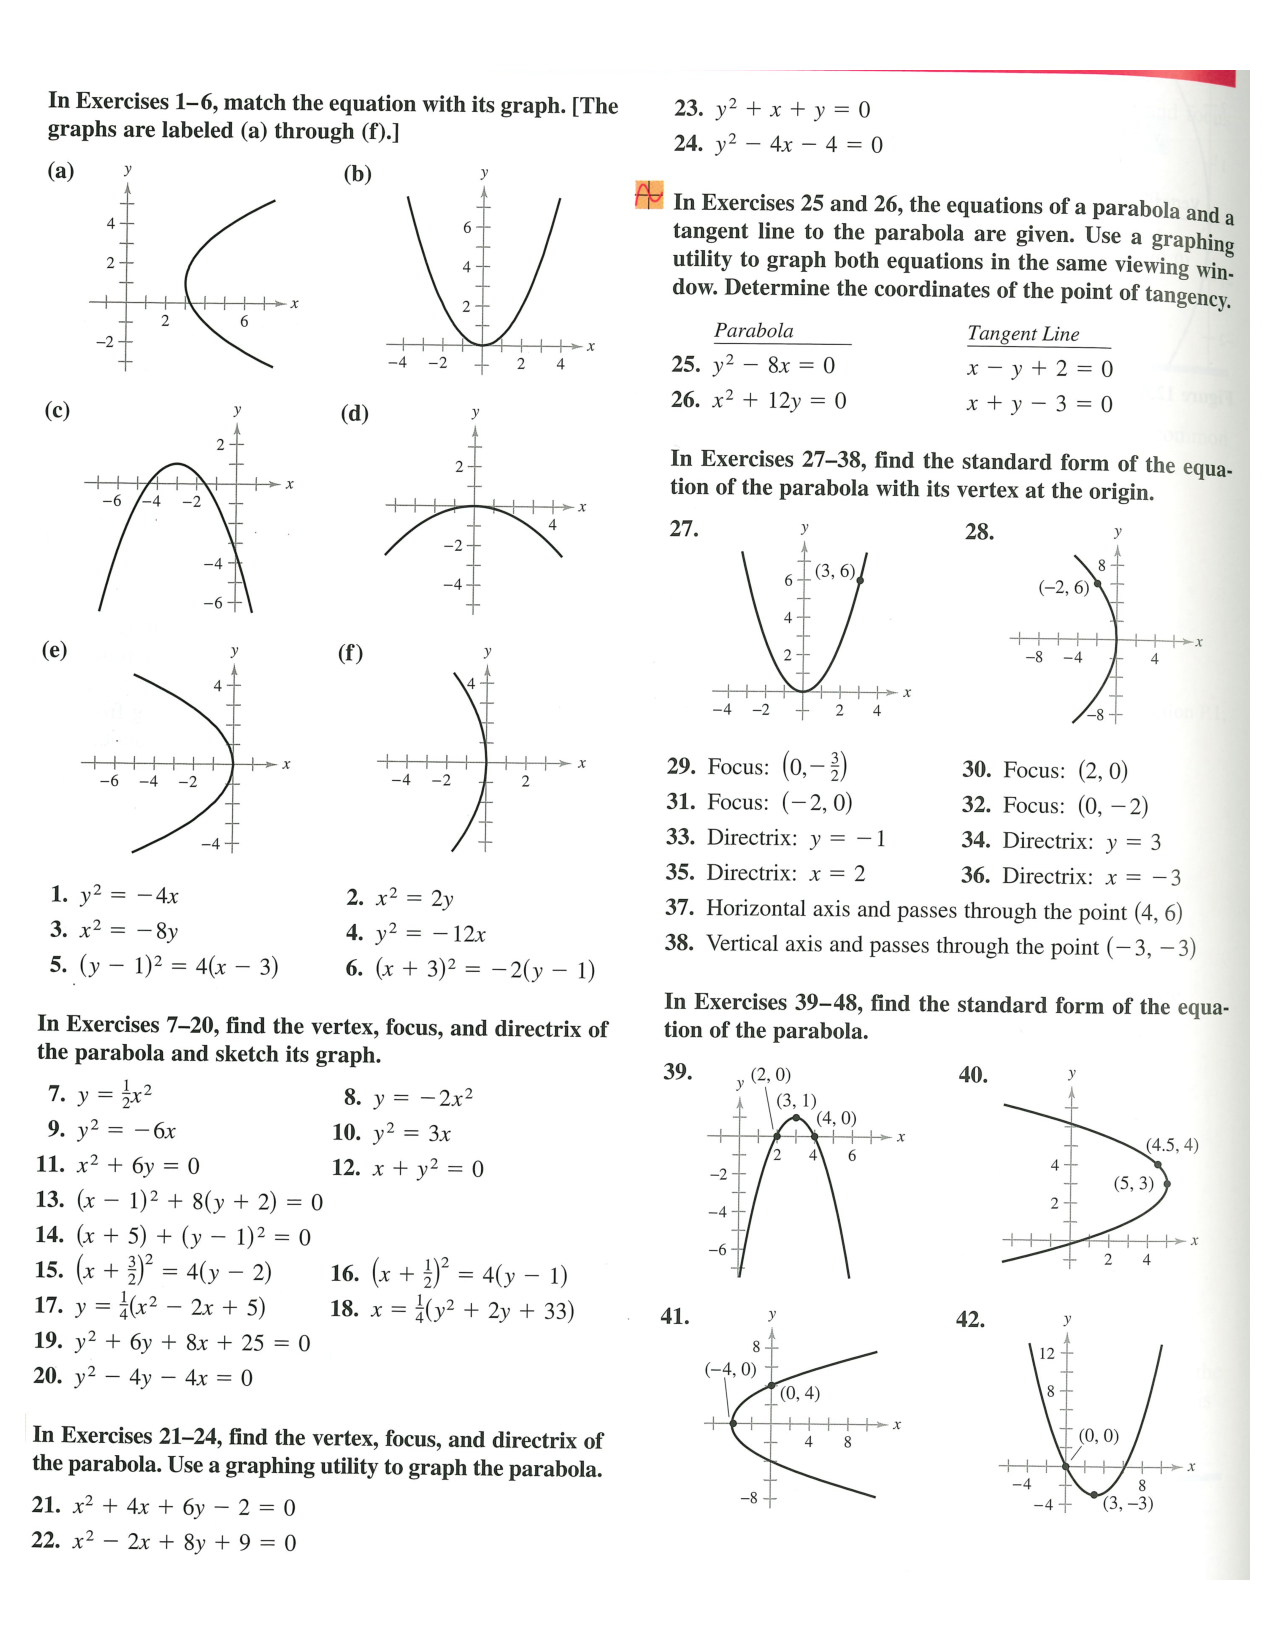
\includegraphics[width=\paperwidth]{\chapdir/0303xA.pdf}}
\newpage
\noindent\makebox[\textwidth]{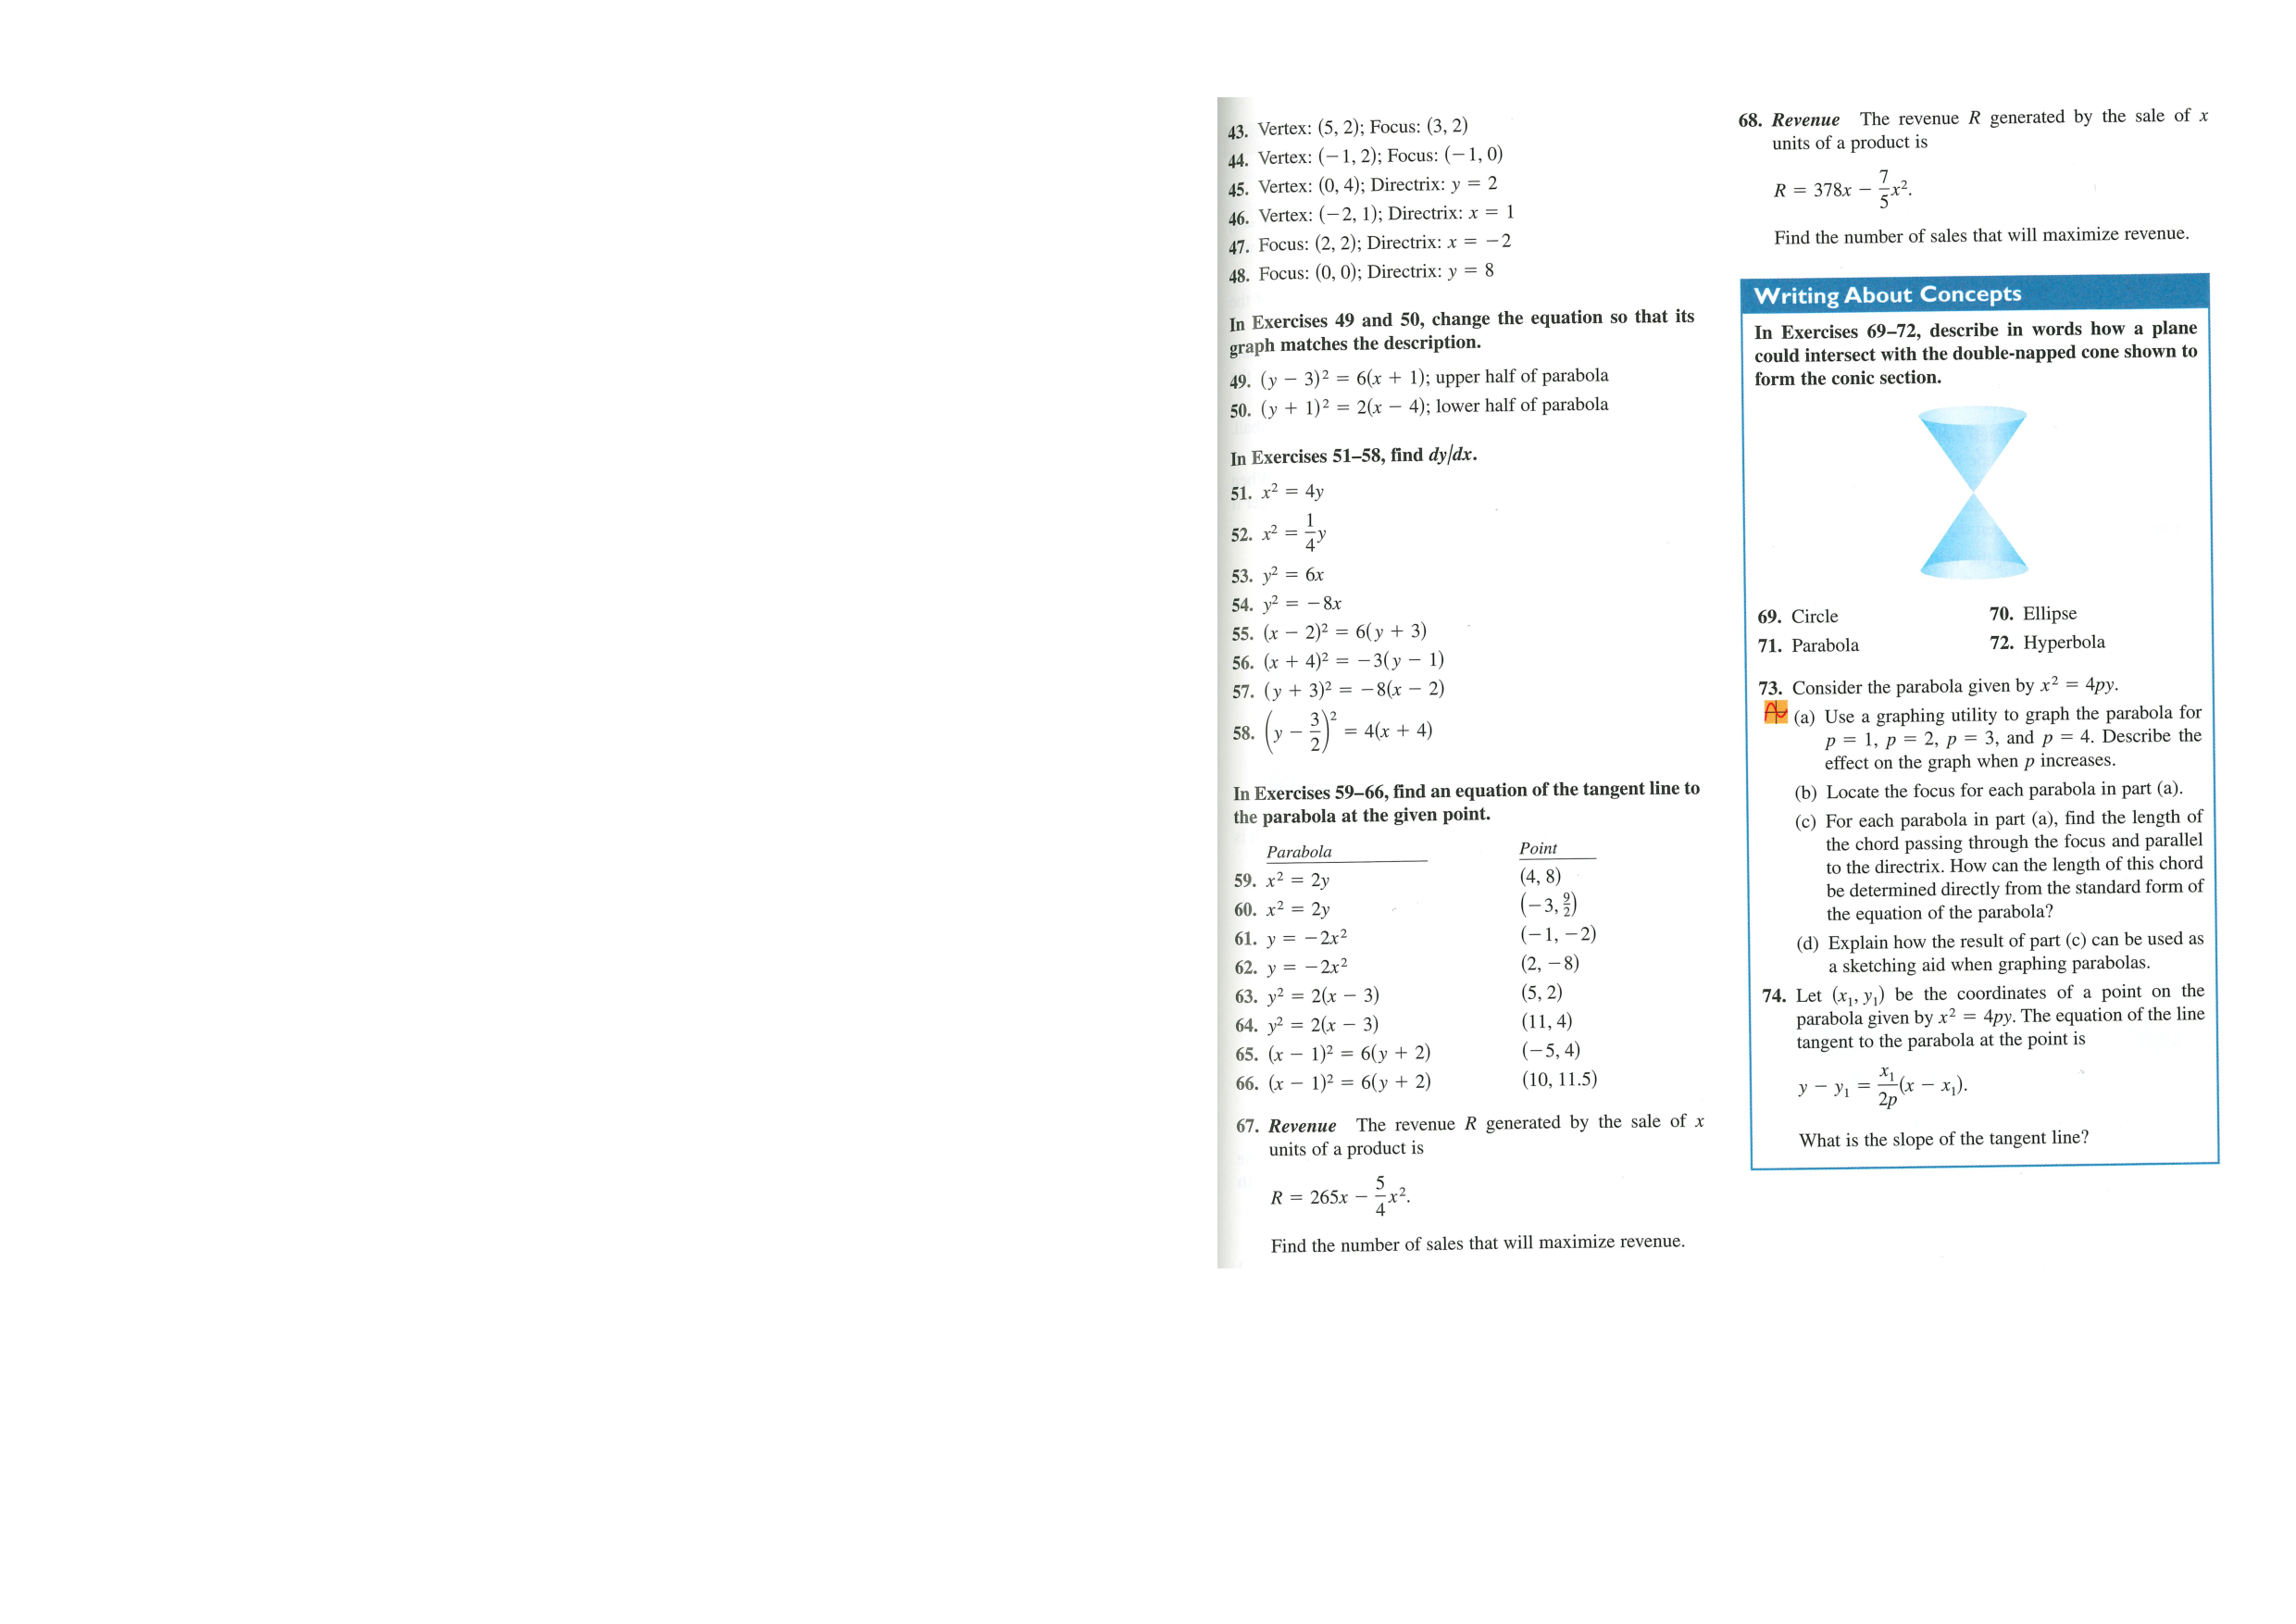
\includegraphics[width=\paperwidth]{\chapdir/0303xB.pdf}}
\newpage
\noindent\makebox[\textwidth]{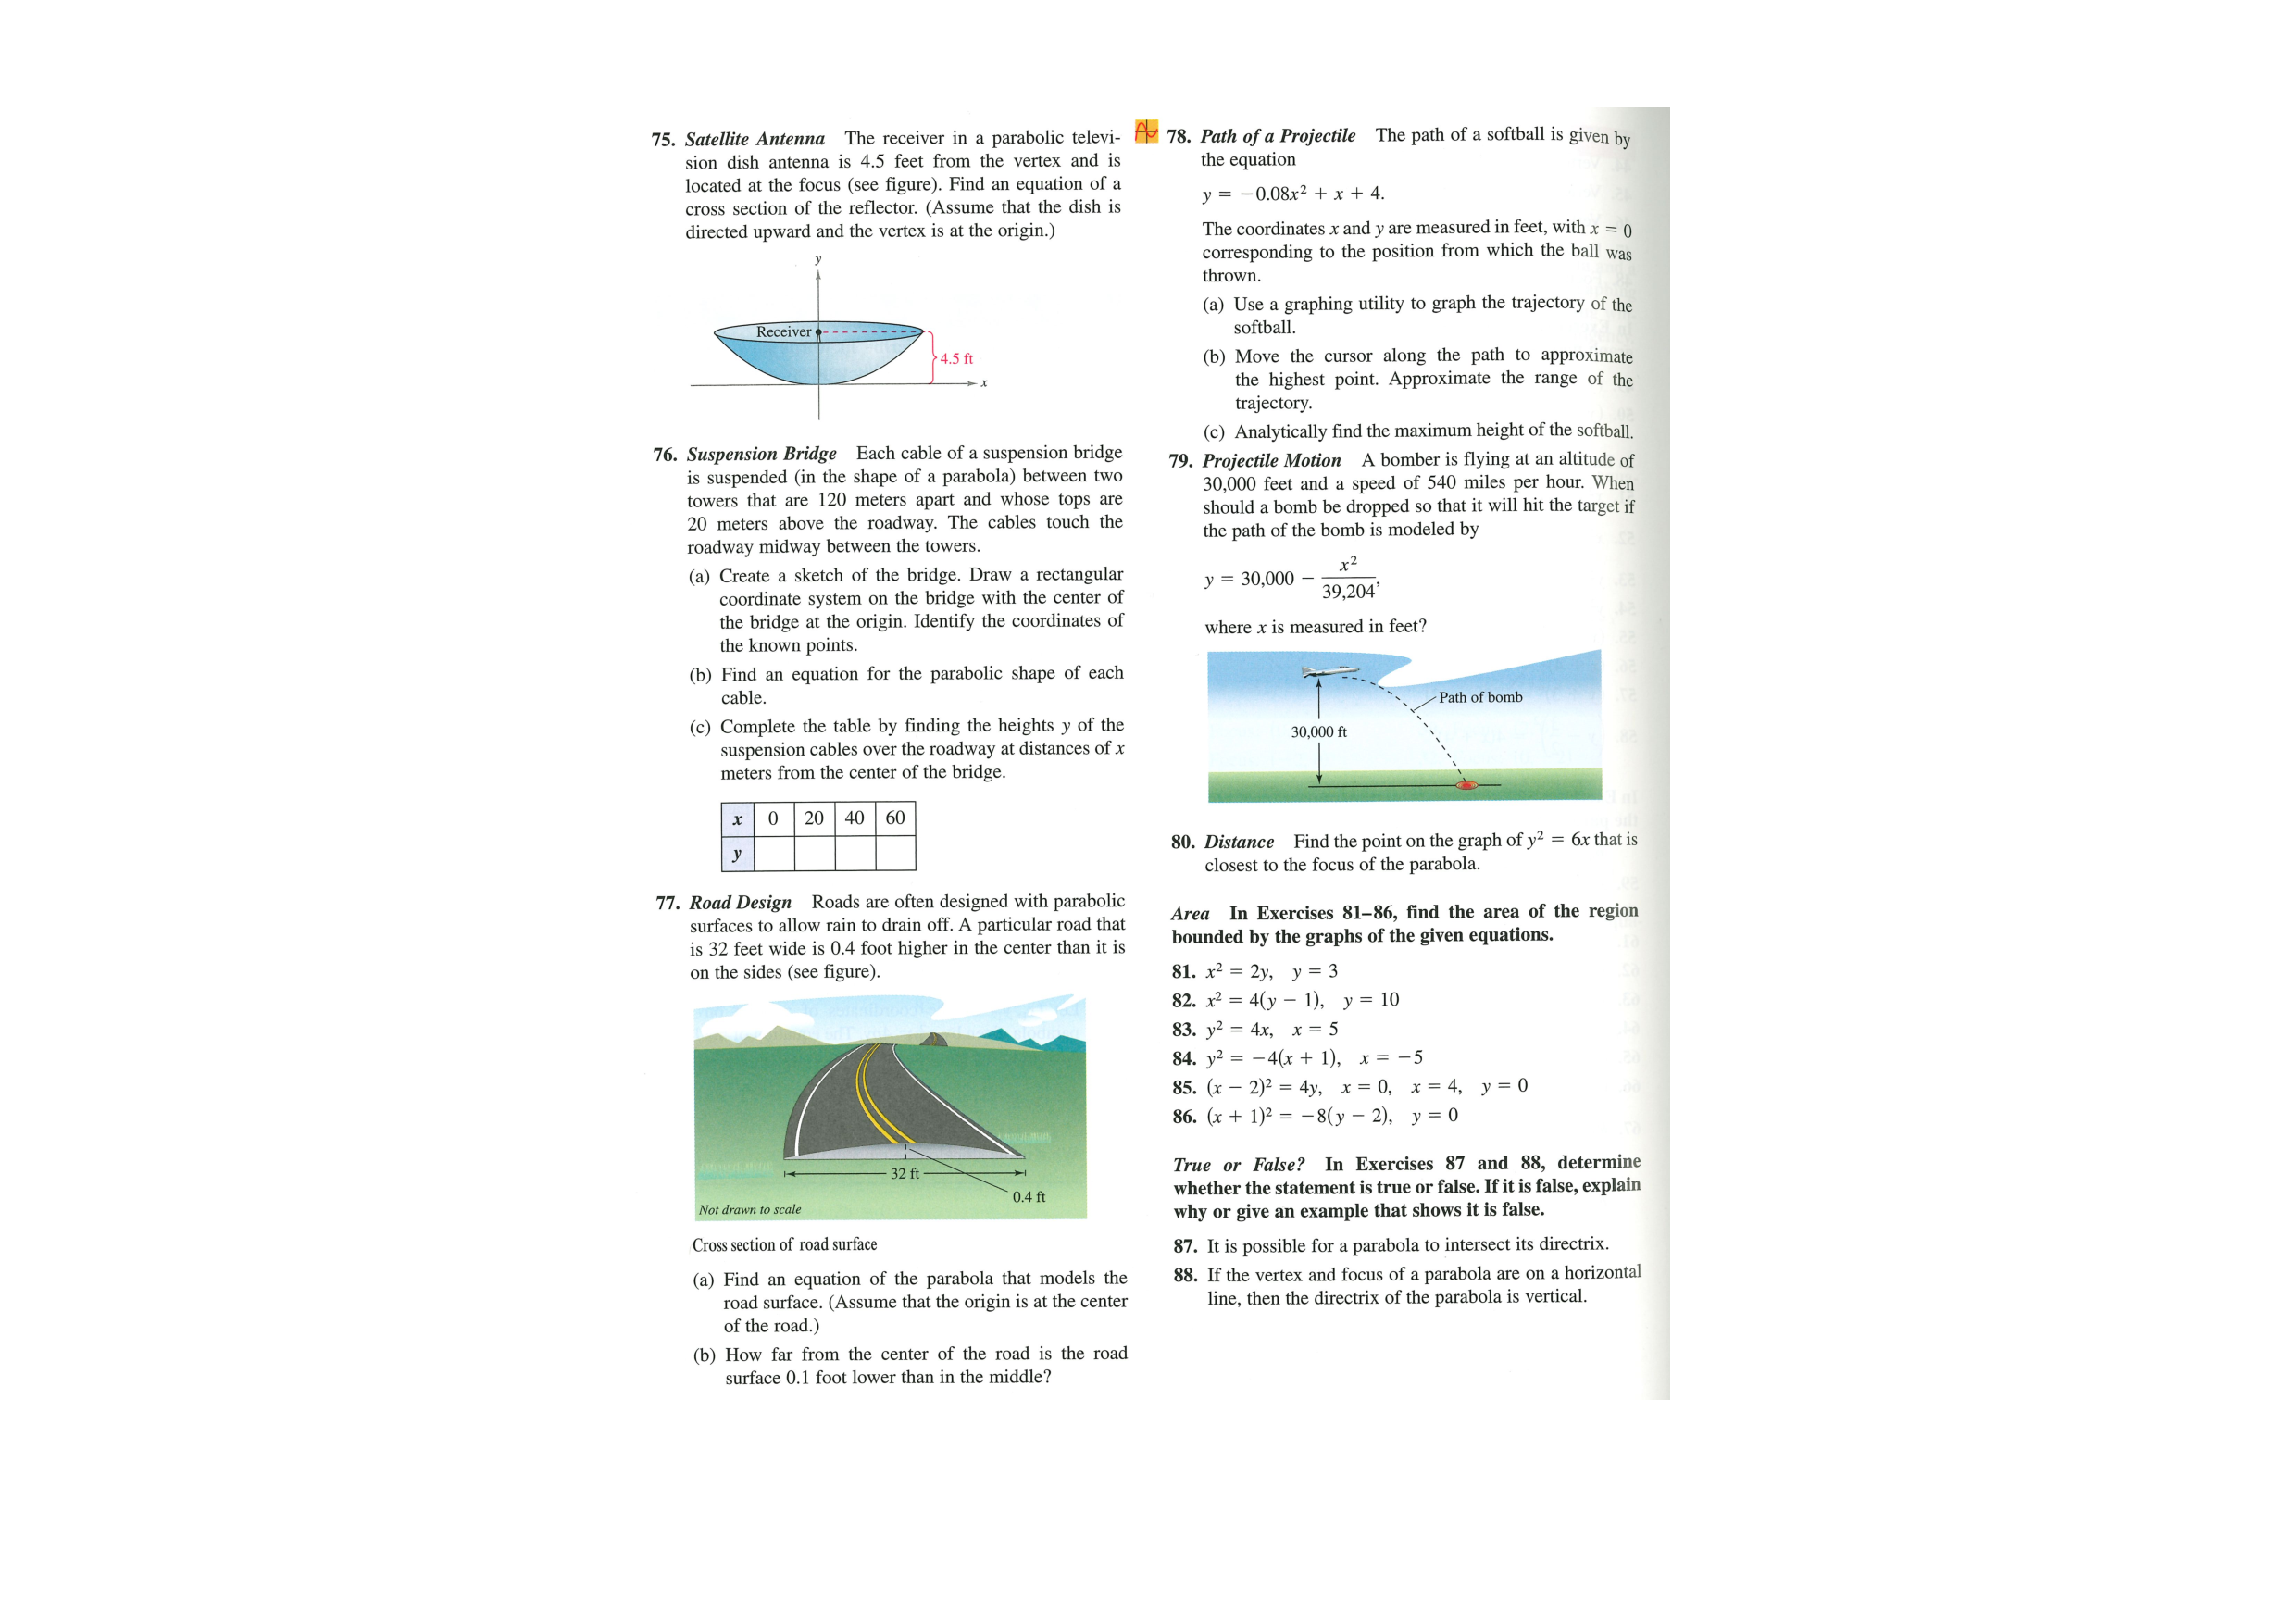
\includegraphics[width=\paperwidth]{\chapdir/0303xC.pdf}}




%							3 - 4
\newpage
\invisiblesection{Radical}
\marginlessinput{\chapdir/0304p}
\newpage
%!TEX root =  ../main.tex

\subsection{Babylonian Method}

\objective{Graph and understand the slope of root functions.}

Square roots are useful whenever someone tell you the square footage of an area.  If it 
were a square, how long would each side be?  Cube roots are similar for volume. 

Dealing with square roots without calculator can be rather intimidating.  But it doesn't have
to be.  3,000 years ago, the Babylonians found a method that truly repays the effort put into it:
each iteration double the number of digits in the estimate!  Few formula converge so quickly.

The square root of $A$:

$R_{n+1}=\cfrac{R_n + \frac{A}{R_n}}{2}$

In short:
\begin{enumerate}
\item Pick the best number you can.
\item Divide the original by ``the number''
\item Average the answer with ``the number''
\item Return to step 2 with this as ``the number''
\end{enumerate}


\subsection{Even vs. Odd}
OK, so you found the square or cube root of some number to as many decimal places as
you need.  Rather than doing \emph{that} more than once, wouldn't it be preferable to find
out how much adding to the inside of a square root changes the output?  In other words,
what is the rate of change, or the derivative?

You will need to multiply top and bottom of the difference quotient by the conjugate of the
numerator.


\begin{example}
\exProblem
A woman rode a train where the cost of train ride is directly proportional to the square 
root of the distance ridden.  Her ticket to ride 140 miles cost \$24.40.  
Find the final per mile rate of a man who got off after 35 miles, 
compared the woman's final rate.

\exSolution
Directly proportional means we can set up an equation $c = k \sqrt{d}$, where $c$ and $d$
are the cost and distance.  If $24.4 = k\sqrt{140}$ then $k=\frac{24.4}{\sqrt{140}}$.  The
derivative of $\frac{24.4}{\sqrt{140}}\sqrt{x} = \frac{12.2}{\sqrt{140x}}$.  At 35, the
derivative is equal to $\frac{24.4}{sqrt{140}} \approx 0.17$, and at 140 it is 
$\frac{12.2}{\sqrt{140}} \approx 0.09$.  This means the woman exited paying over
\$0.08 less per mile than the man.
\end{example}

~\vfill

~\vfill
\subsection{Exercises}
\noindent\makebox[\textwidth]{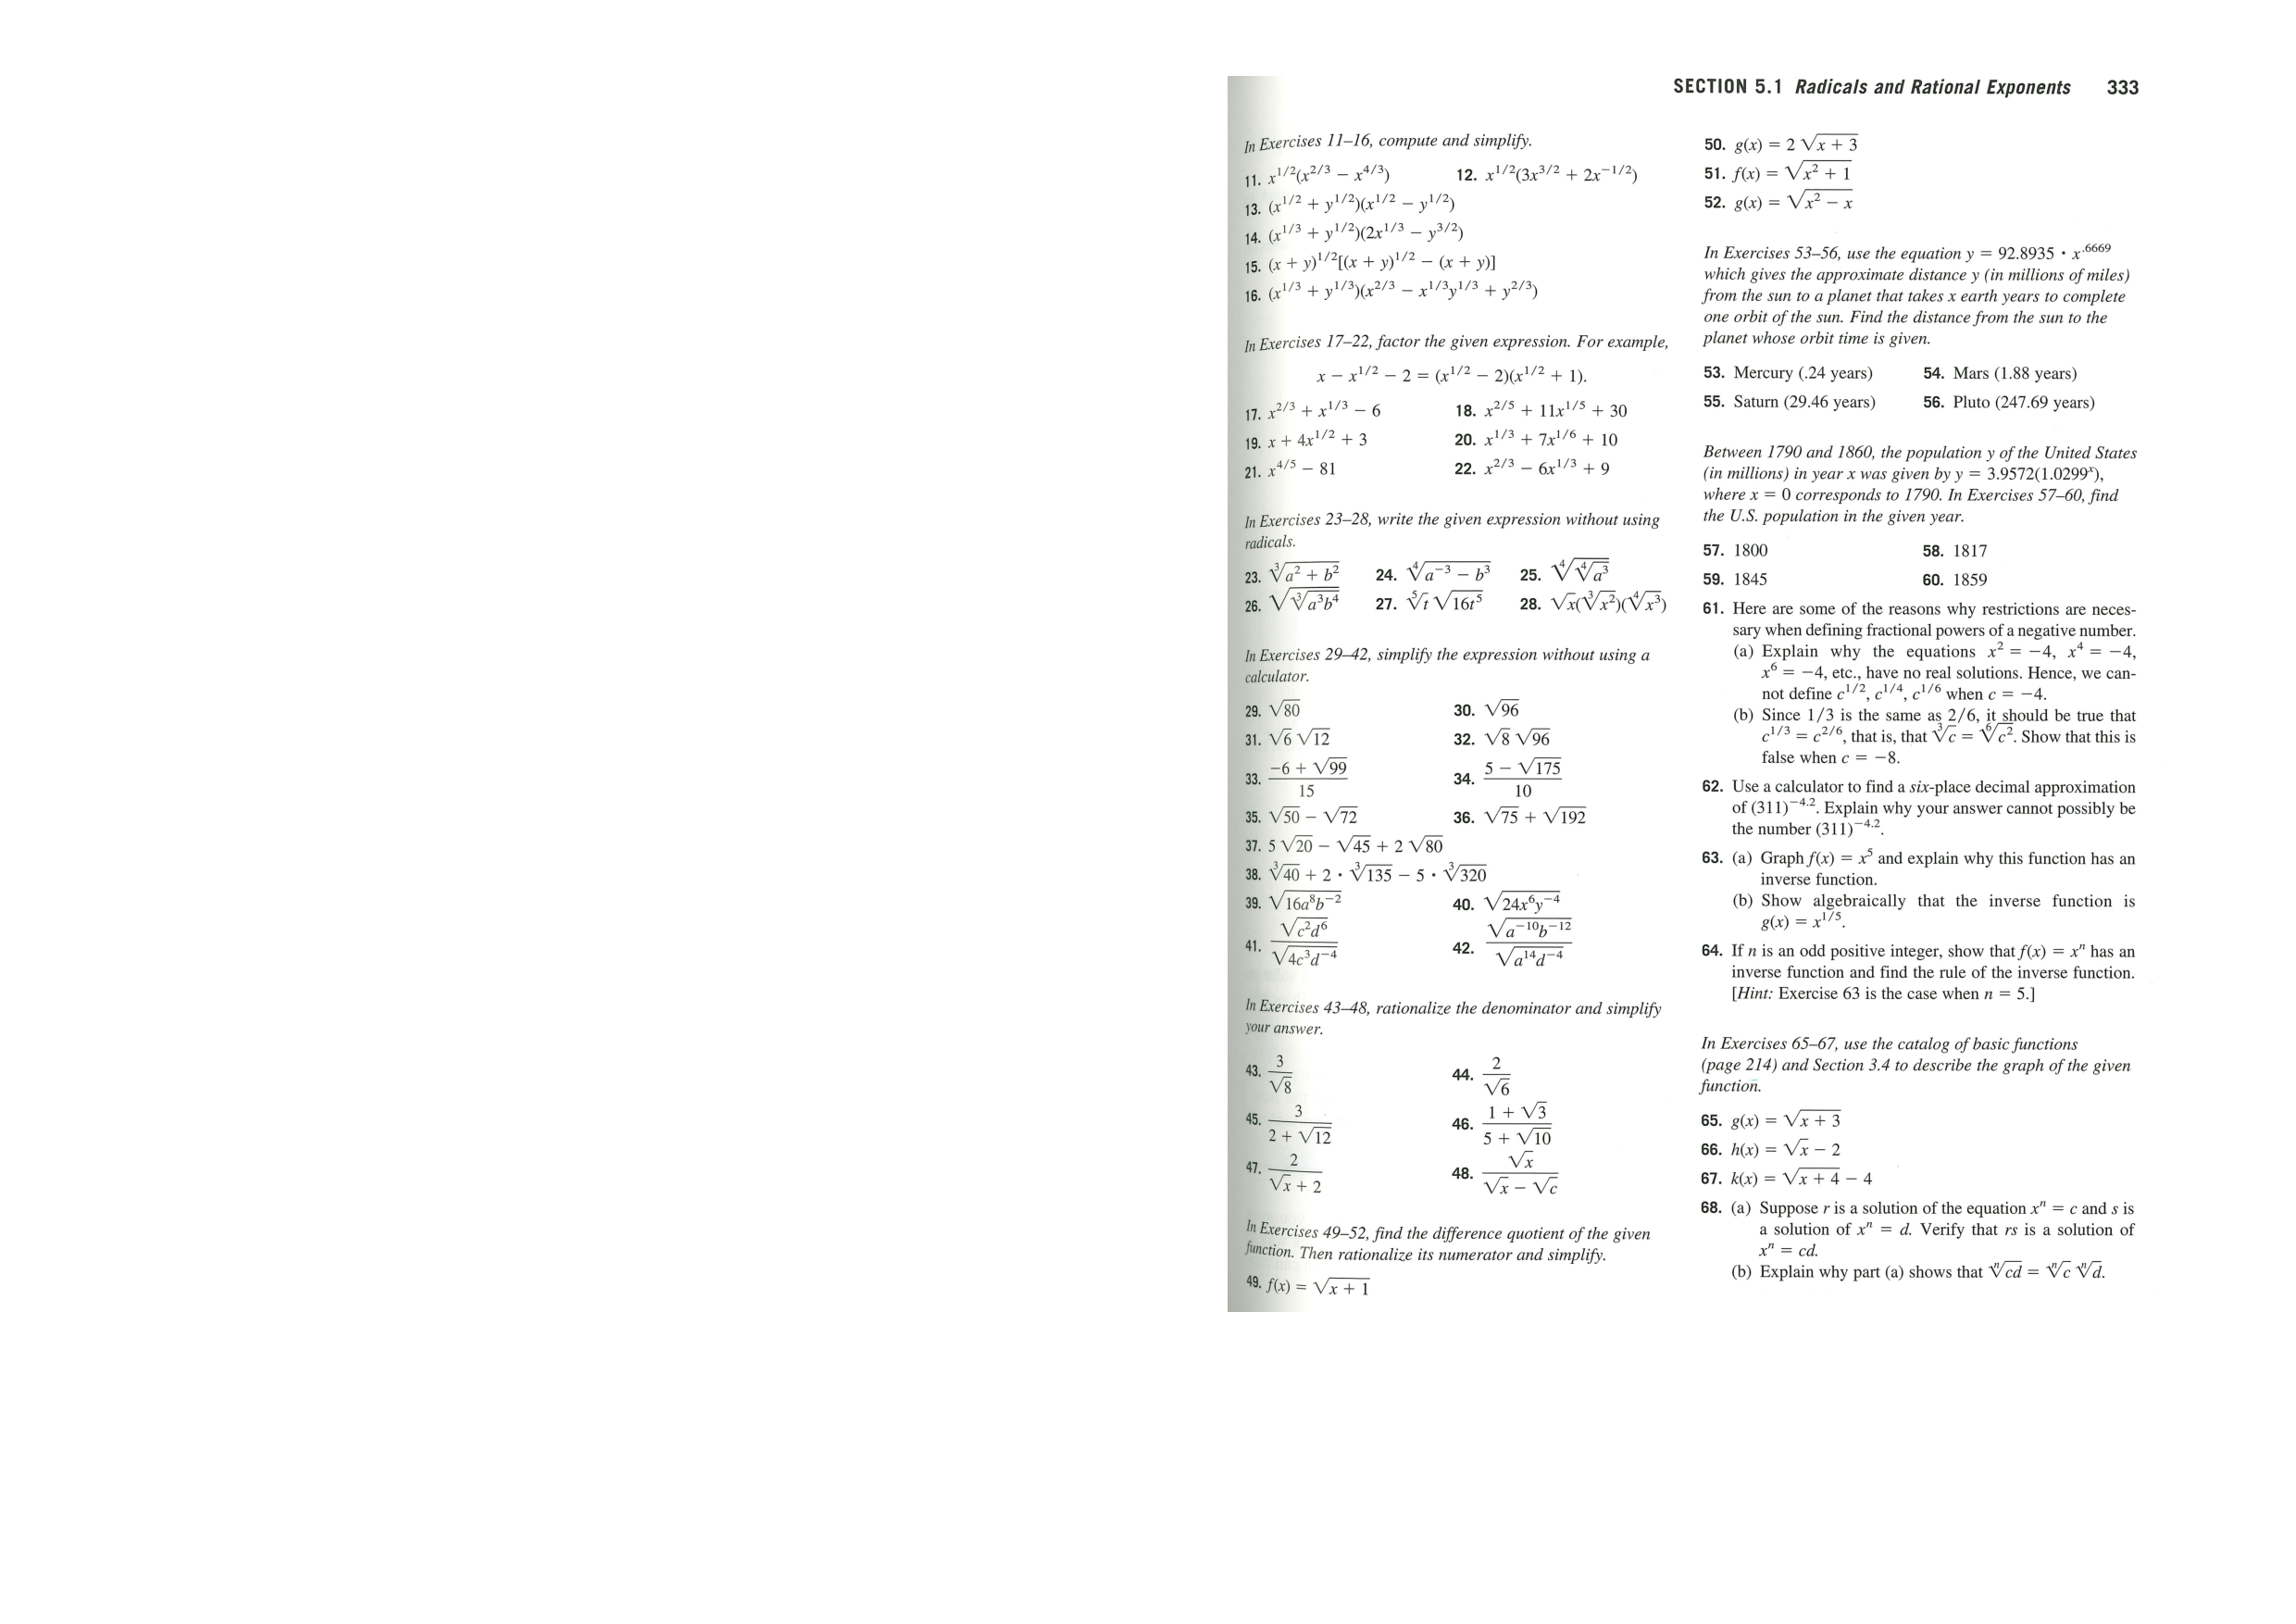
\includegraphics[width=\paperwidth]{\chapdir/0304xA.pdf}}
newpage
\noindent\makebox[\textwidth]{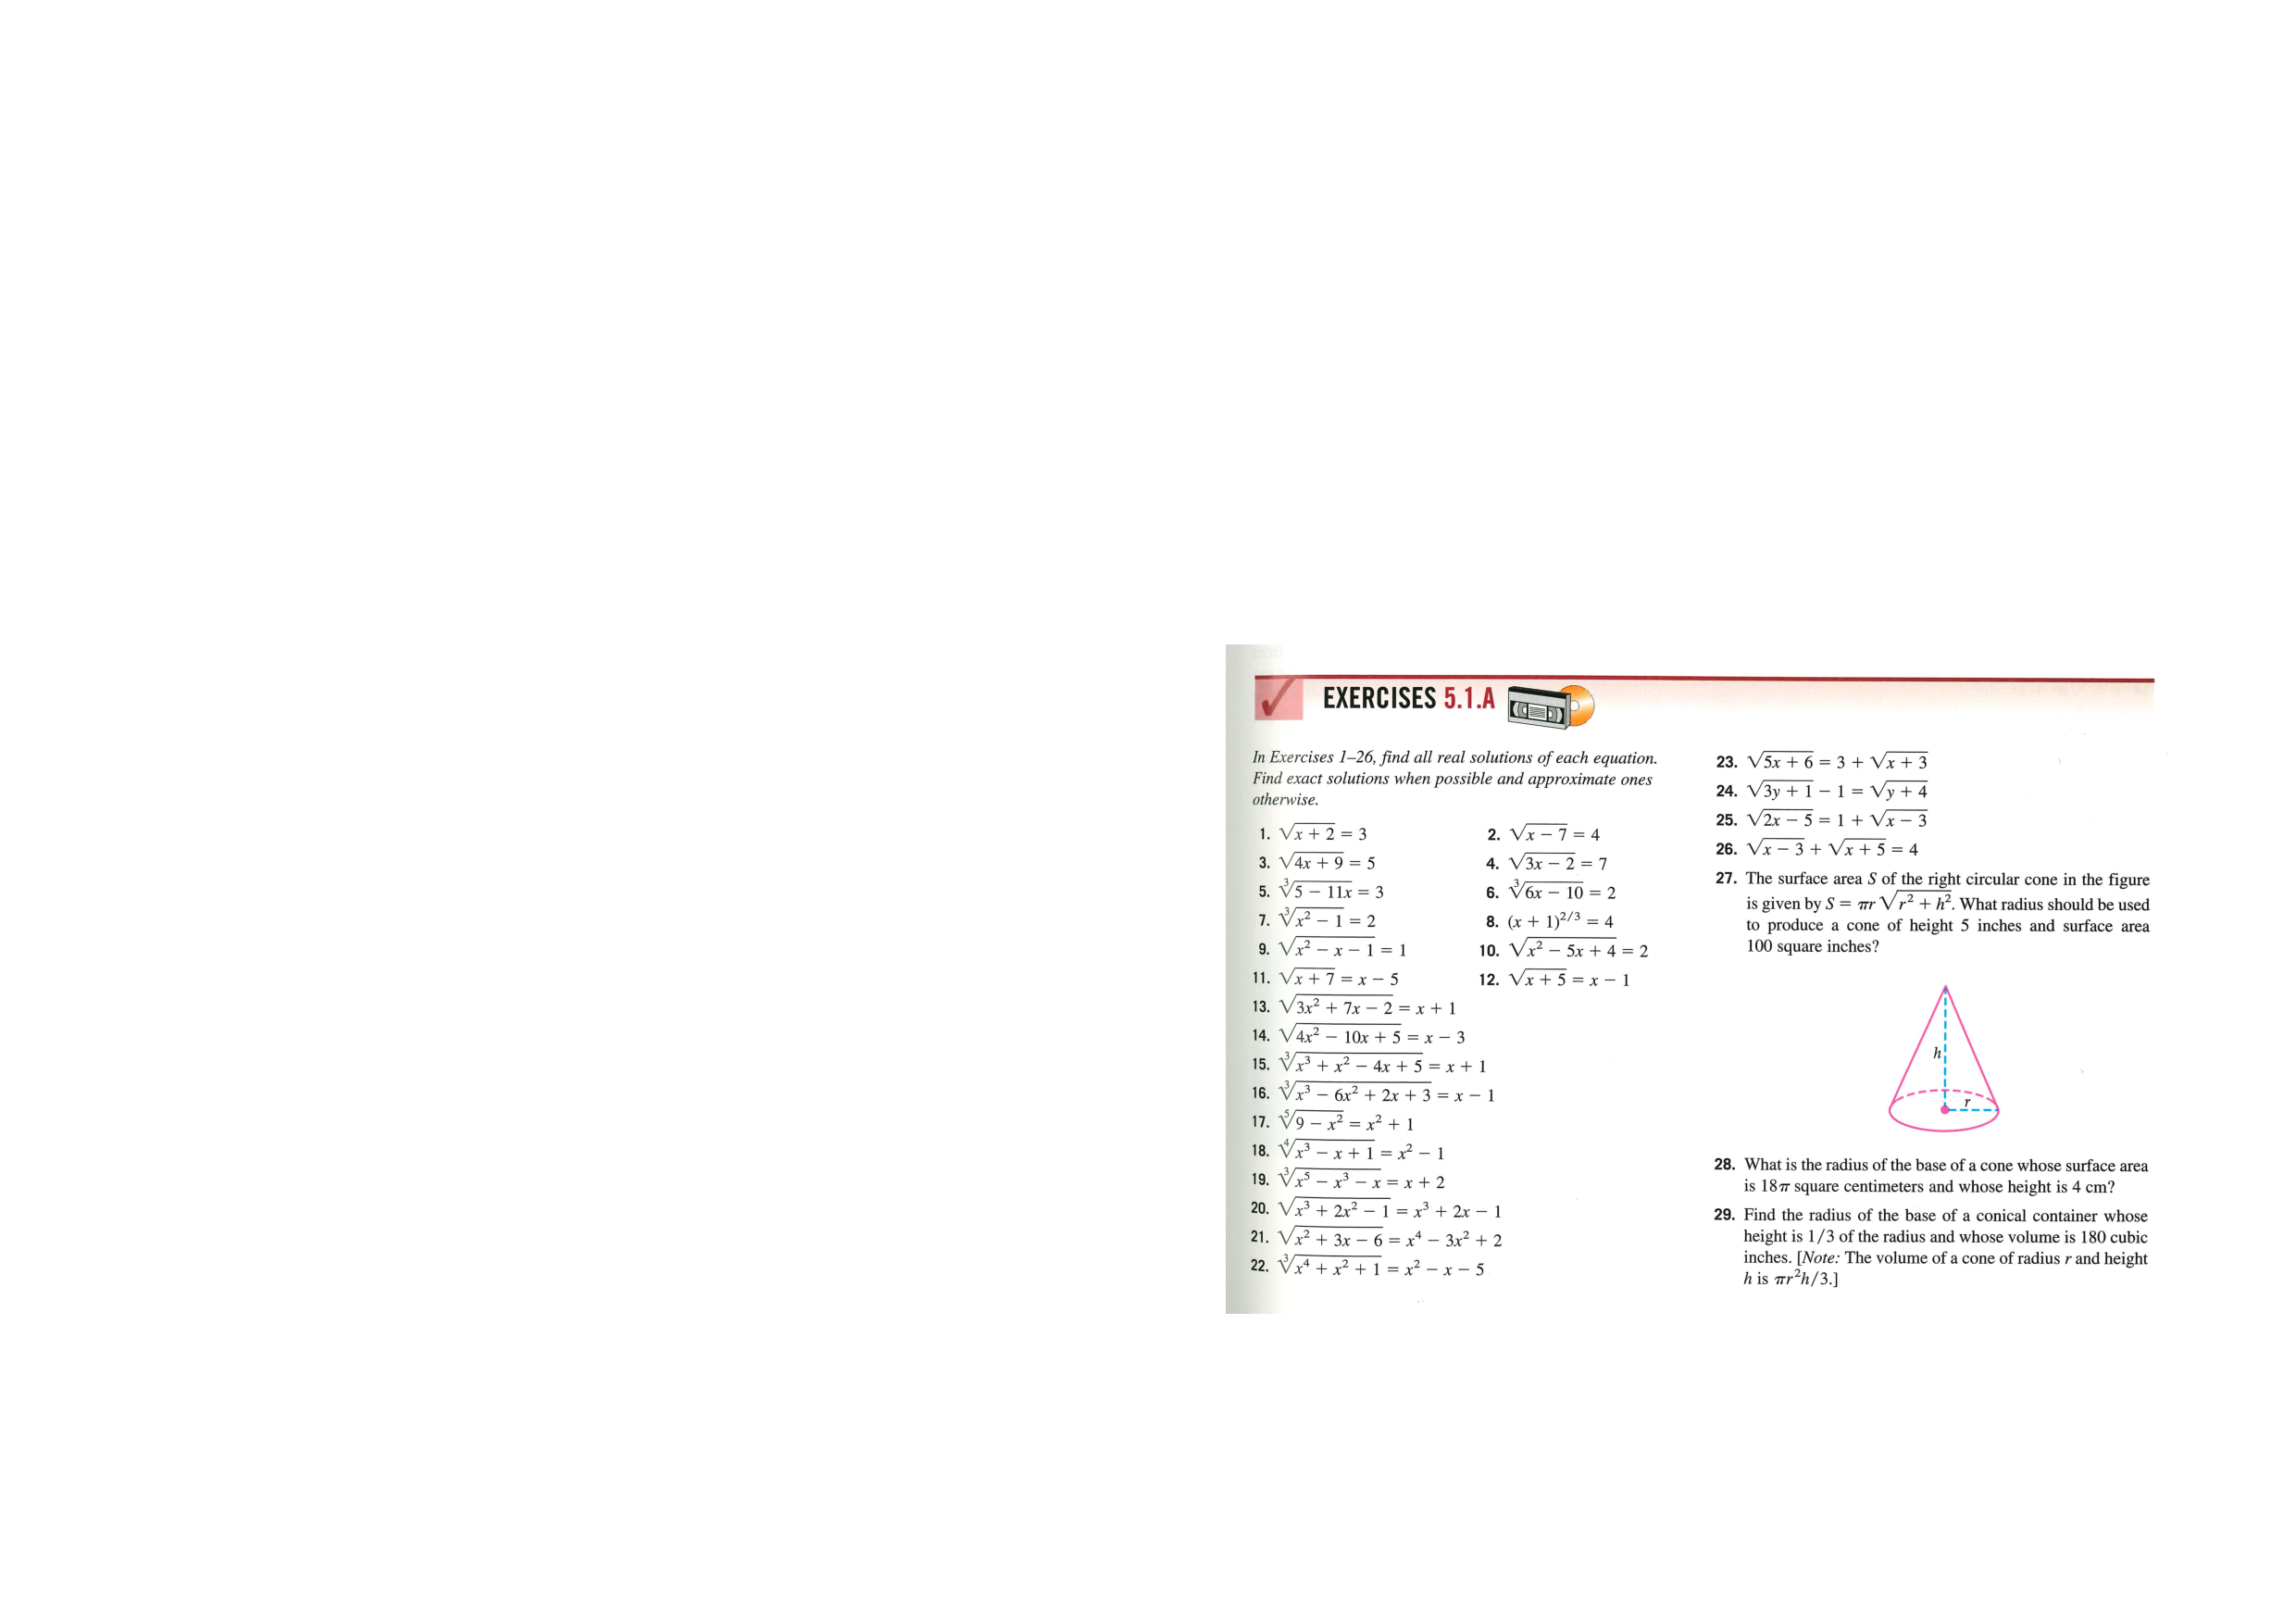
\includegraphics[width=\paperwidth]{\chapdir/0304xB.pdf}}
\newpage
\noindent\makebox[\textwidth]{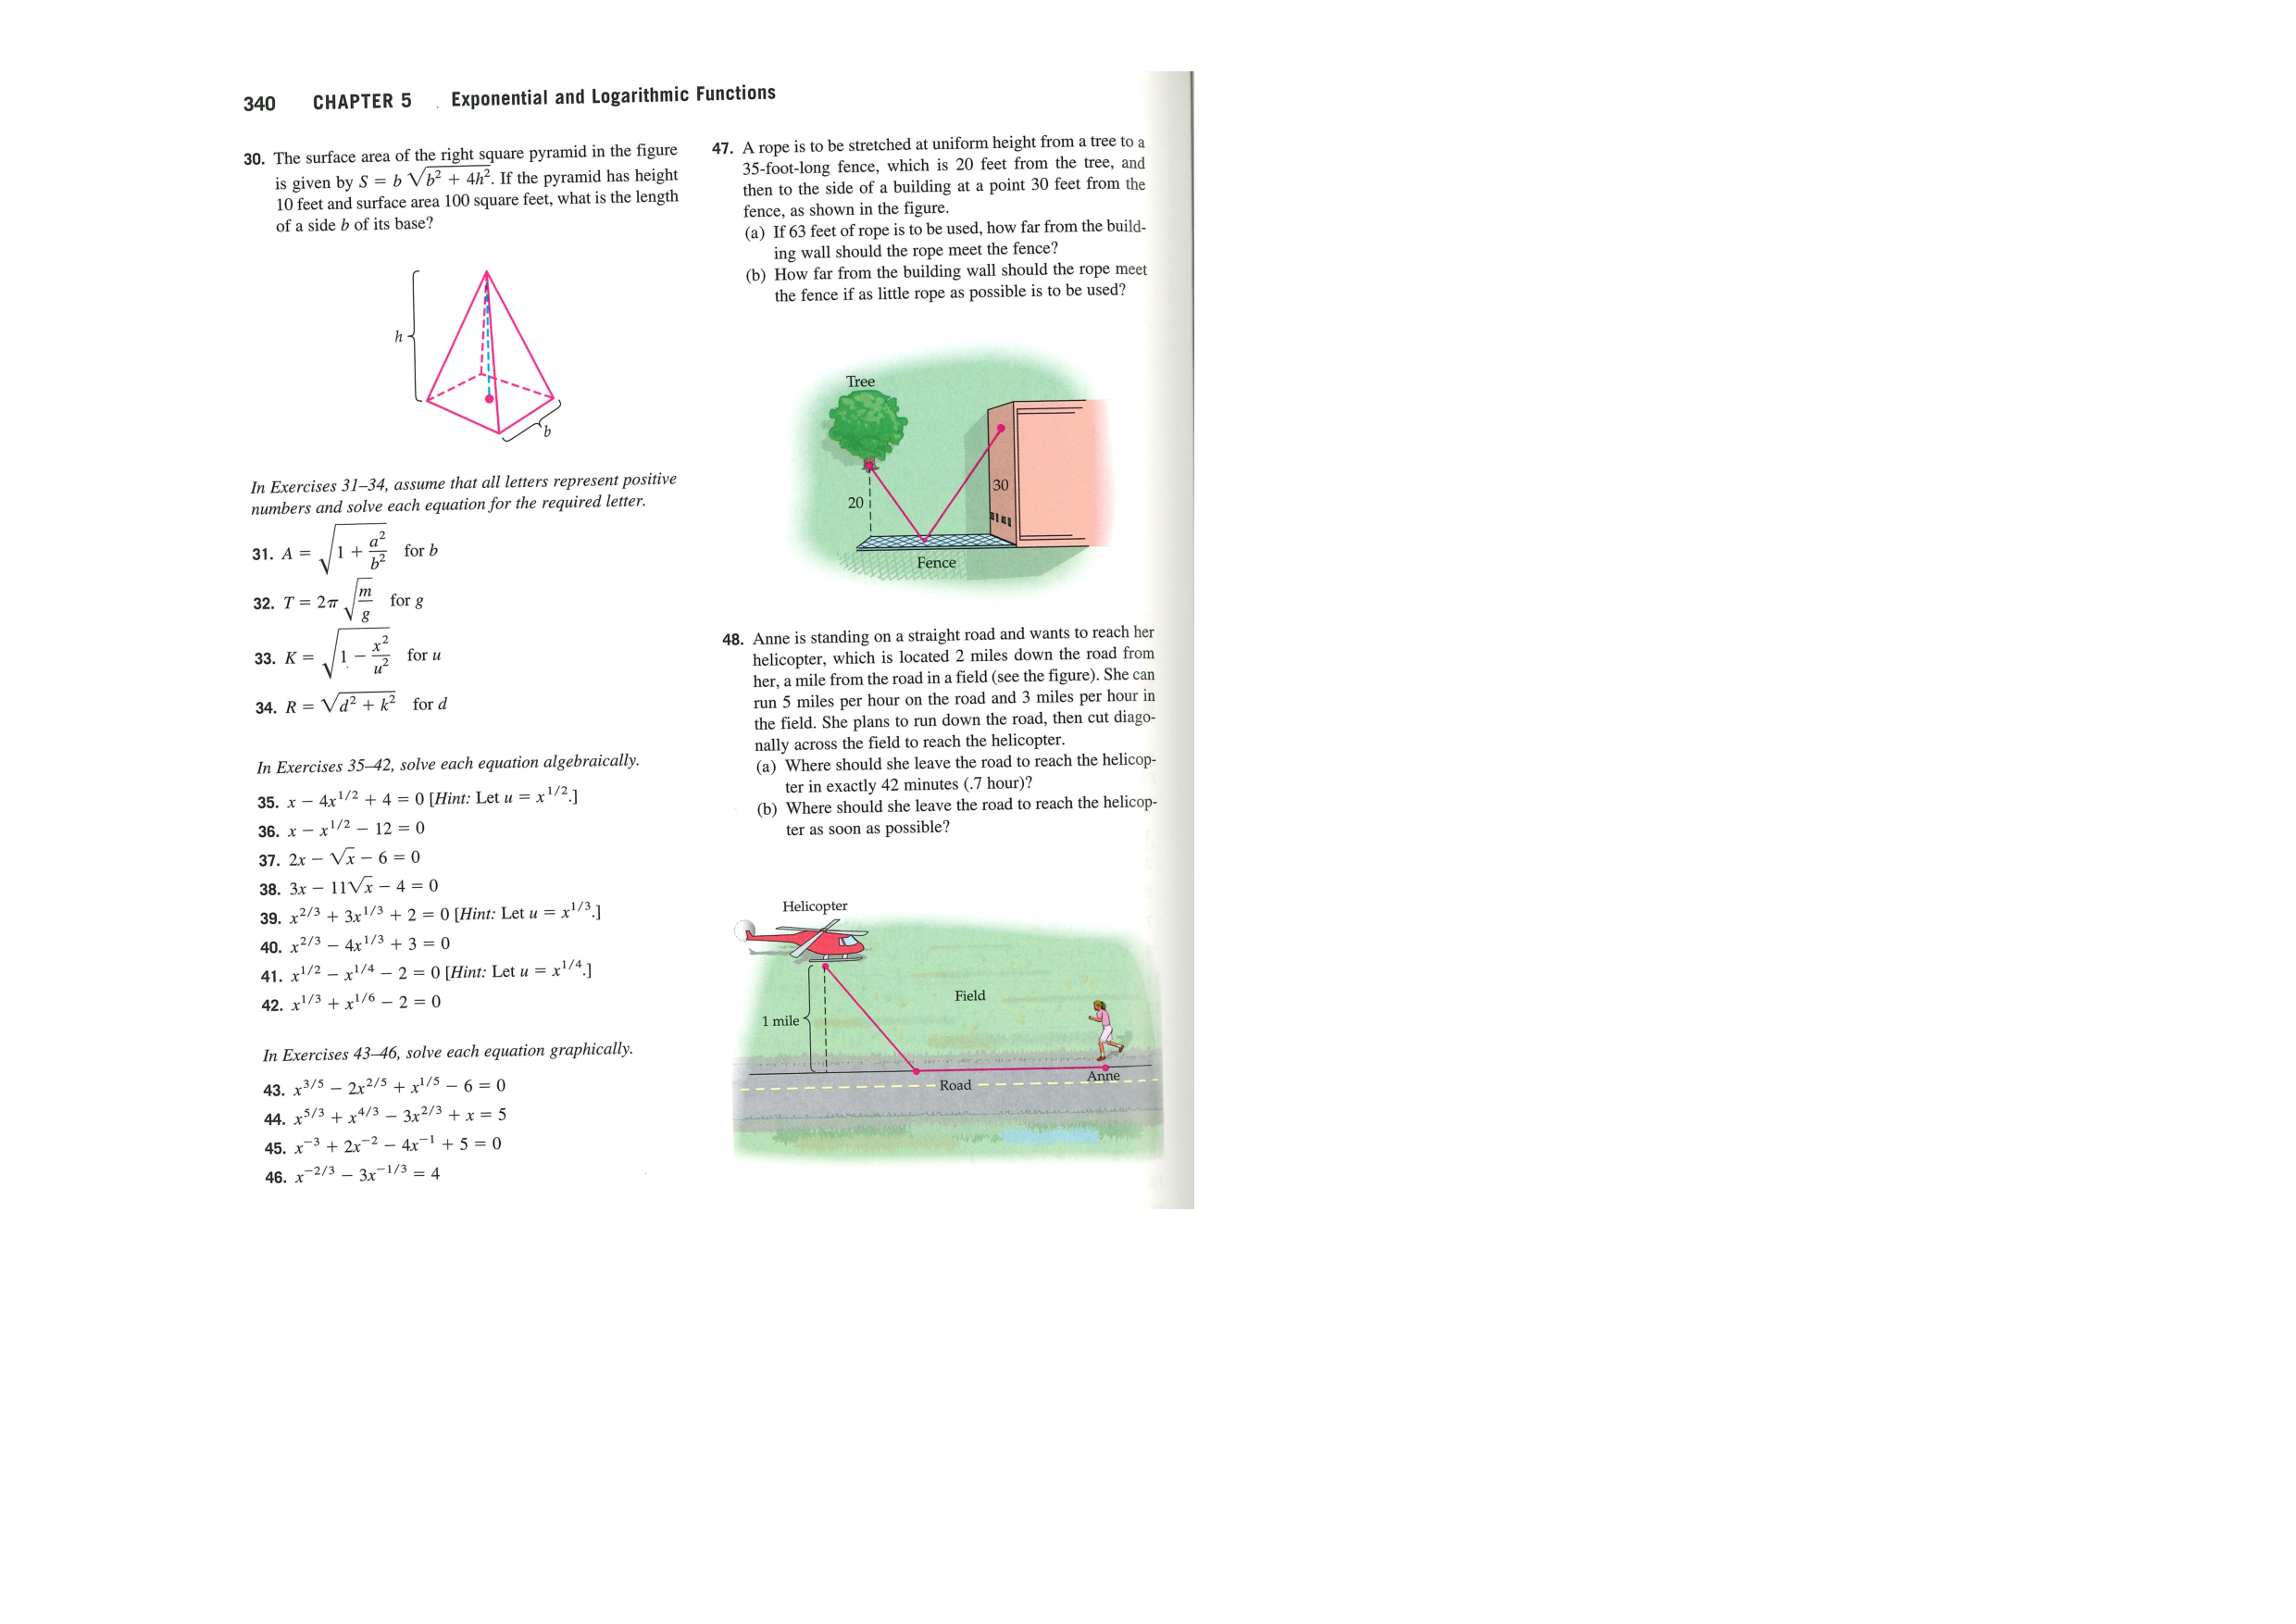
\includegraphics[width=\paperwidth]{\chapdir/0304xC.pdf}}
\newpage
\noindent\makebox[\textwidth]{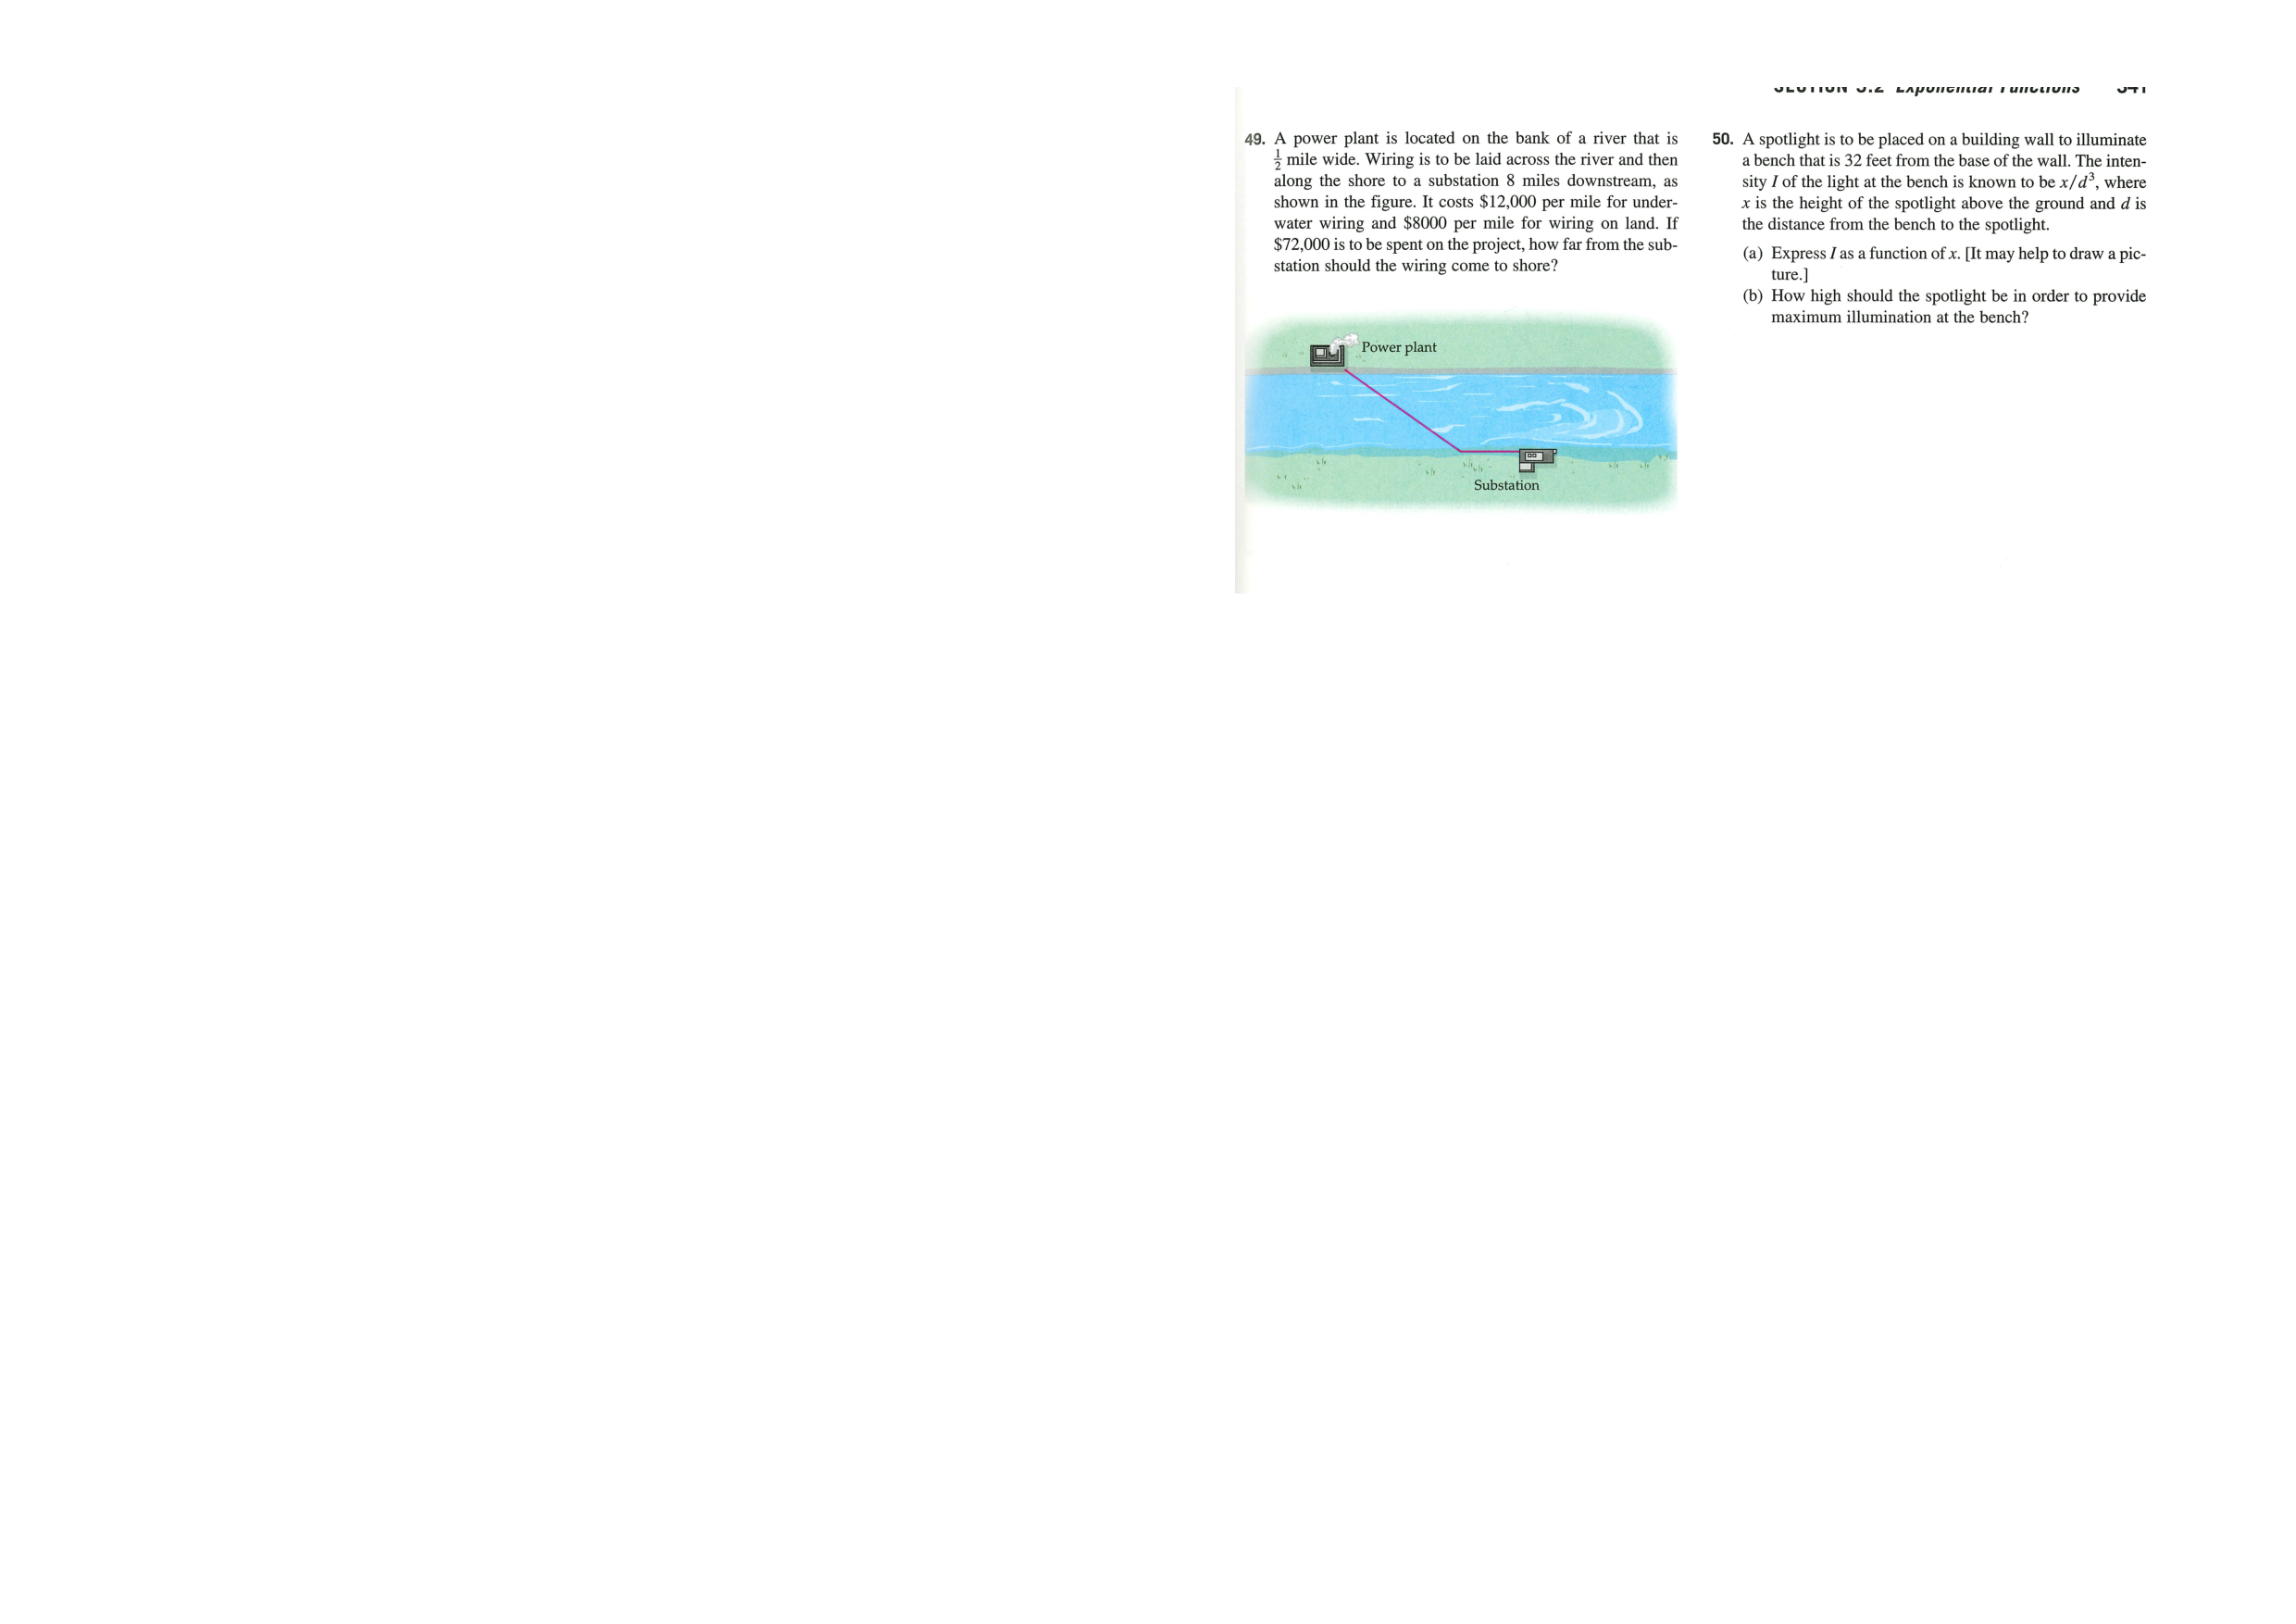
\includegraphics[width=\paperwidth]{\chapdir/0304xD.pdf}}




%							3 - 5
%\newpage
\invisiblesection{Derivatives}
%\subsection{Problems}
\noindent\makebox[\textwidth]{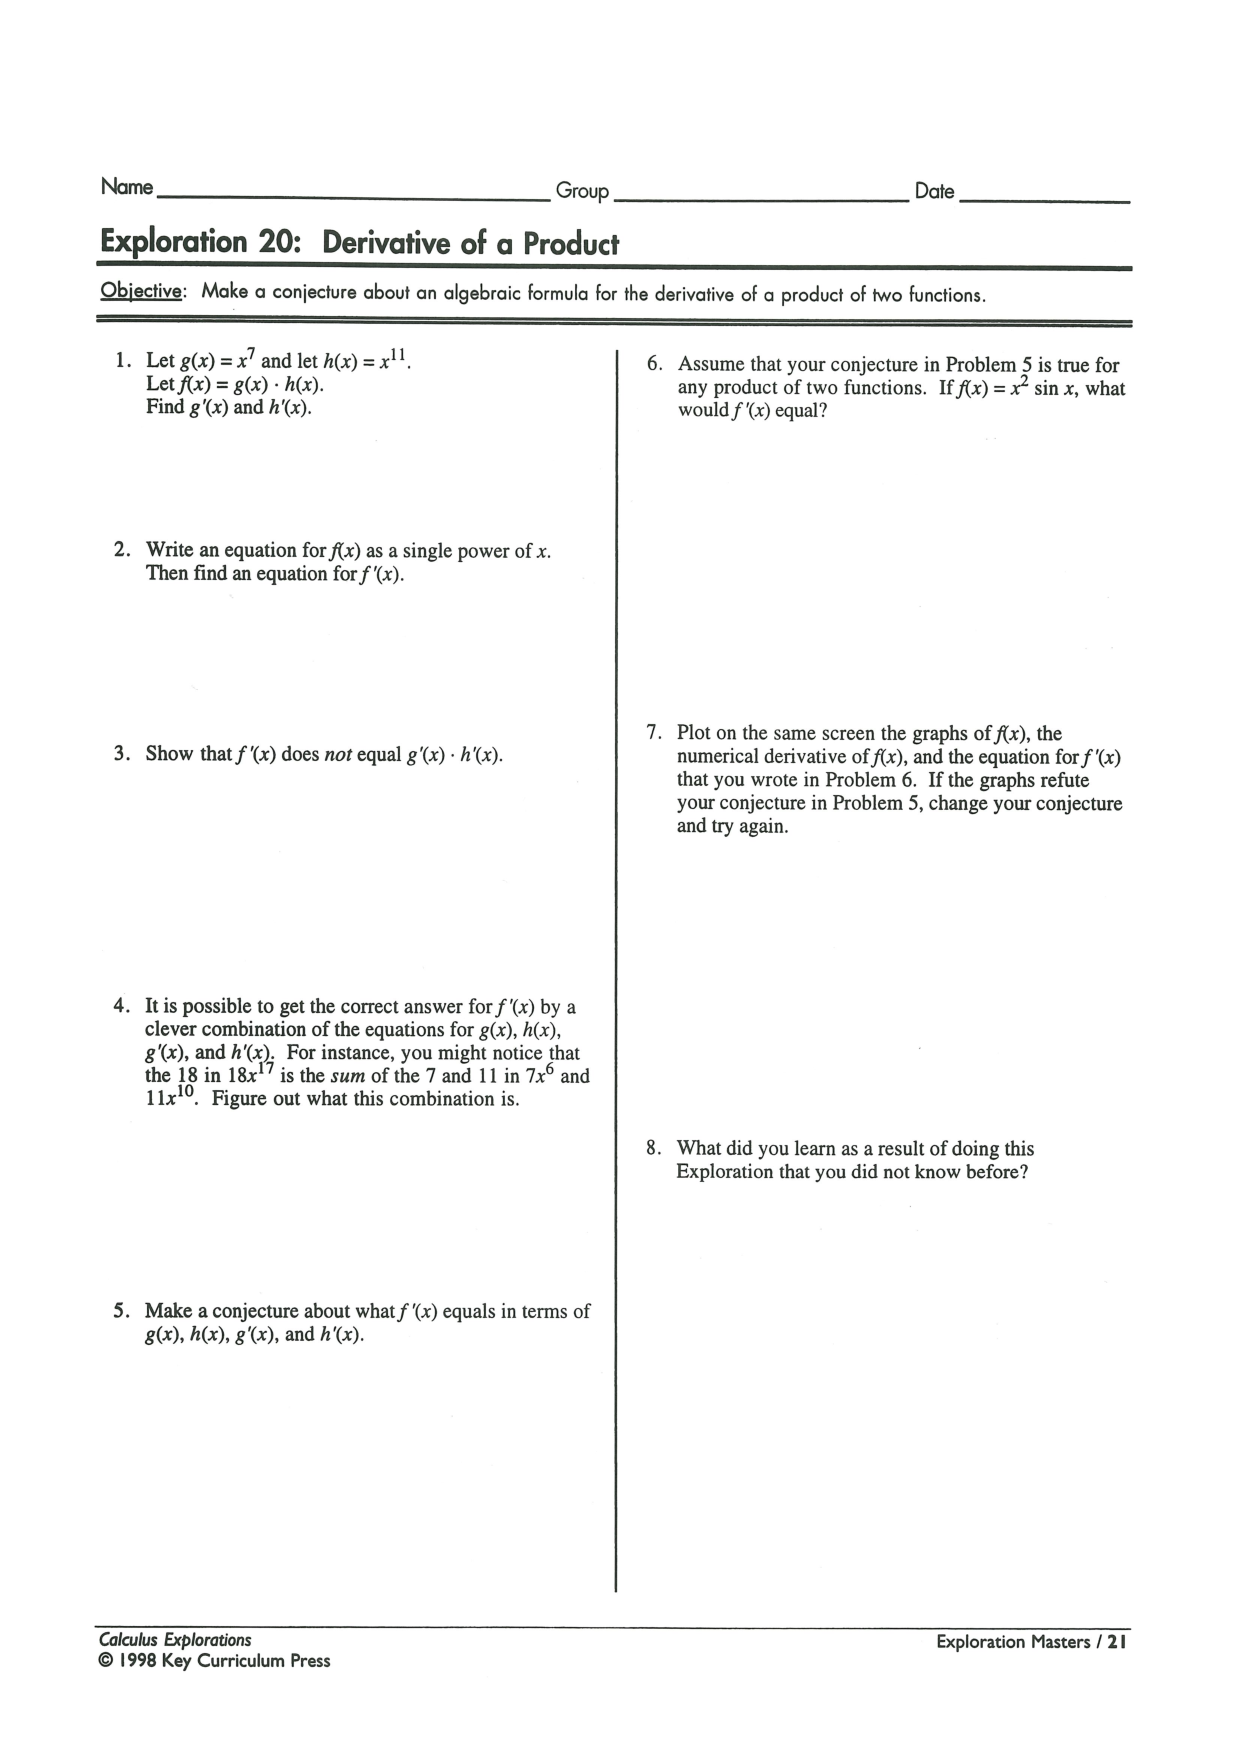
\includegraphics[width=\paperwidth]{\chapdir/0305p.pdf}}
\newpage
%!TEX root =  ../main.tex

\subsection{Properties of Derivatives}

\objective{Calculate derivates using the Power, Product, and Quotient Rules.}


\index{Derivative!properties}
The derivative of a sum of two functions is the sum of the derivatives of each function.

The derivative of a constant times a function is the constant times the derivative of the function.

The derivative of a constant is 0.

\subsubsection{Product Rule (inductive)}
\index{Product Rule}\index{Derivative!of a product}
The following proof is very arbitrary and does not feel like something anyone would try
unprompted (especially in the second line: who would ever think of adding and subtracting the same
term in just that way?!).  We will use the following \textbf{Product Rule} some over the coming chapters,
but a full proof that you are responsible for reproducing does not come until §8.3

\begin{align*}
  (fg)'(x) & = \lim_{h\rightarrow0}\frac{f(x+h)g(x+h) - f(x)g(x)}{h} \\
  	&= \lim_{h\rightarrow0}\frac{f(x+h)g(x+h) - f(x)g(x+h) + f(x)g(x+h) + f(x)g(x)}{h} \\
	&= \lim_{h\rightarrow0}\frac{f(x+h)g(x+h) - f(x)g(x+h)}{h} + \lim_{h\rightarrow0}\frac{f(x)g(x+h)-f(x)g(x)}{h} \\
	&= \lim_{h\rightarrow0}\left[\frac{f(x+h) - f(x)}{h} \cdot g(x+h)\right] + \lim_{h\rightarrow0}\left[\frac{g(x+h)-g(x)}{h} \cdot f(x)\right] \\
	&= \lim_{h\rightarrow0}\left[\frac{f(x+h) - f(x)}{h}\right] \cdot g(x) + \lim_{h\rightarrow0}\left[\frac{g(x+h)-g(x)}{h}\right] \cdot f(x)\\
	&=f'(x)g(x) + f(x)g'(x)
\end{align*}

\subsubsection{Quotient Rule}
\index{Quotient Rule}\index{Derivative!of a quotient}
The \textbf{Quotient Rule} is presented here with a very similar arbitrary trick.  Wait to memorize the proof until chapter 8.

\begin{align*}
\frac{f}{g}' & = \lim_{h\rightarrow0}\cfrac{\frac{f(x+h)}{g(x+h)}-\frac{f(x)}{g(x)}}{h} \\
	&=  \lim_{h\rightarrow0}\frac{g(x)f(x+h)-f(x)g(x+h)}{g(x)g(x+h)h} \\
	&=  \lim_{h\rightarrow0}\frac{g(x)f(x+h)-f(x)g(x)+f(x)g(x)-f(x)g(x+h)}{g(x)g(x+h)h} \\
	&=  g(x)\left[\lim_{h\rightarrow0}\frac{1}{g(x)g(x+h)}\cdot{}\frac{f(x+h)-f(x)}{h}\right]-f(x)\left[\lim_{h\rightarrow0}\frac{1}{g(x)g(x+h)}\cdot{}\frac{g(x+h)-g(x)}{h}\right] \\
	&= \frac{g(x)f'(x) - f(x)g'(x)}{[g(x)]^2}
\end{align*}

\subsection{Power Rule}
\index{Power Rule}\index{Derivative!of a power}
The algebraic derivative of $x^n$ is $n\cdot x^{n-1}$.  While we will furnish a systematic proof 
later (also in section 8.3), we have seen enough inductive
examples of the \textbf{Power Rule} in this chapter
that you are formally responsible for knowing it and using it in all cases.
~\vfill
%\newpage
\subsection{Exercises}
\noindent\makebox[\textwidth]{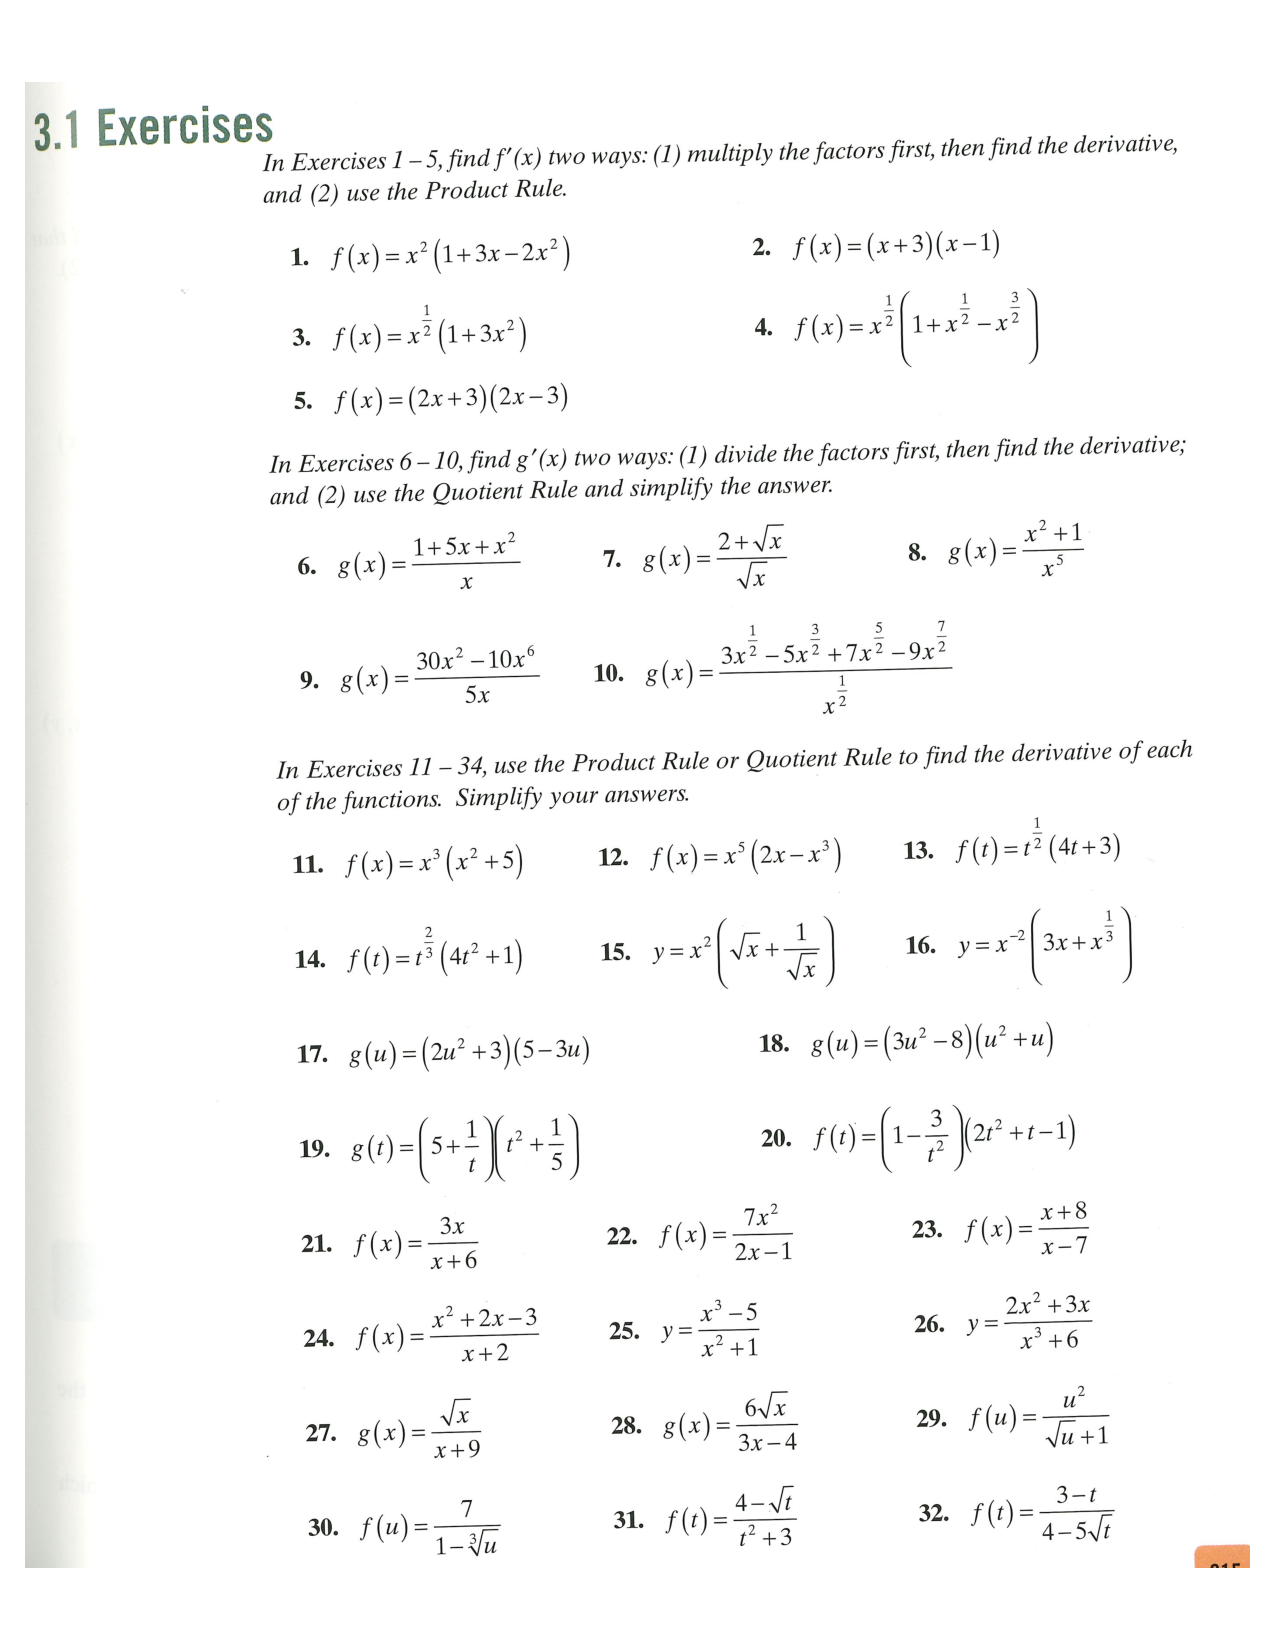
\includegraphics[width=\paperwidth]{\chapdir/0305xA.pdf}}
\newpage
\noindent\makebox[\textwidth]{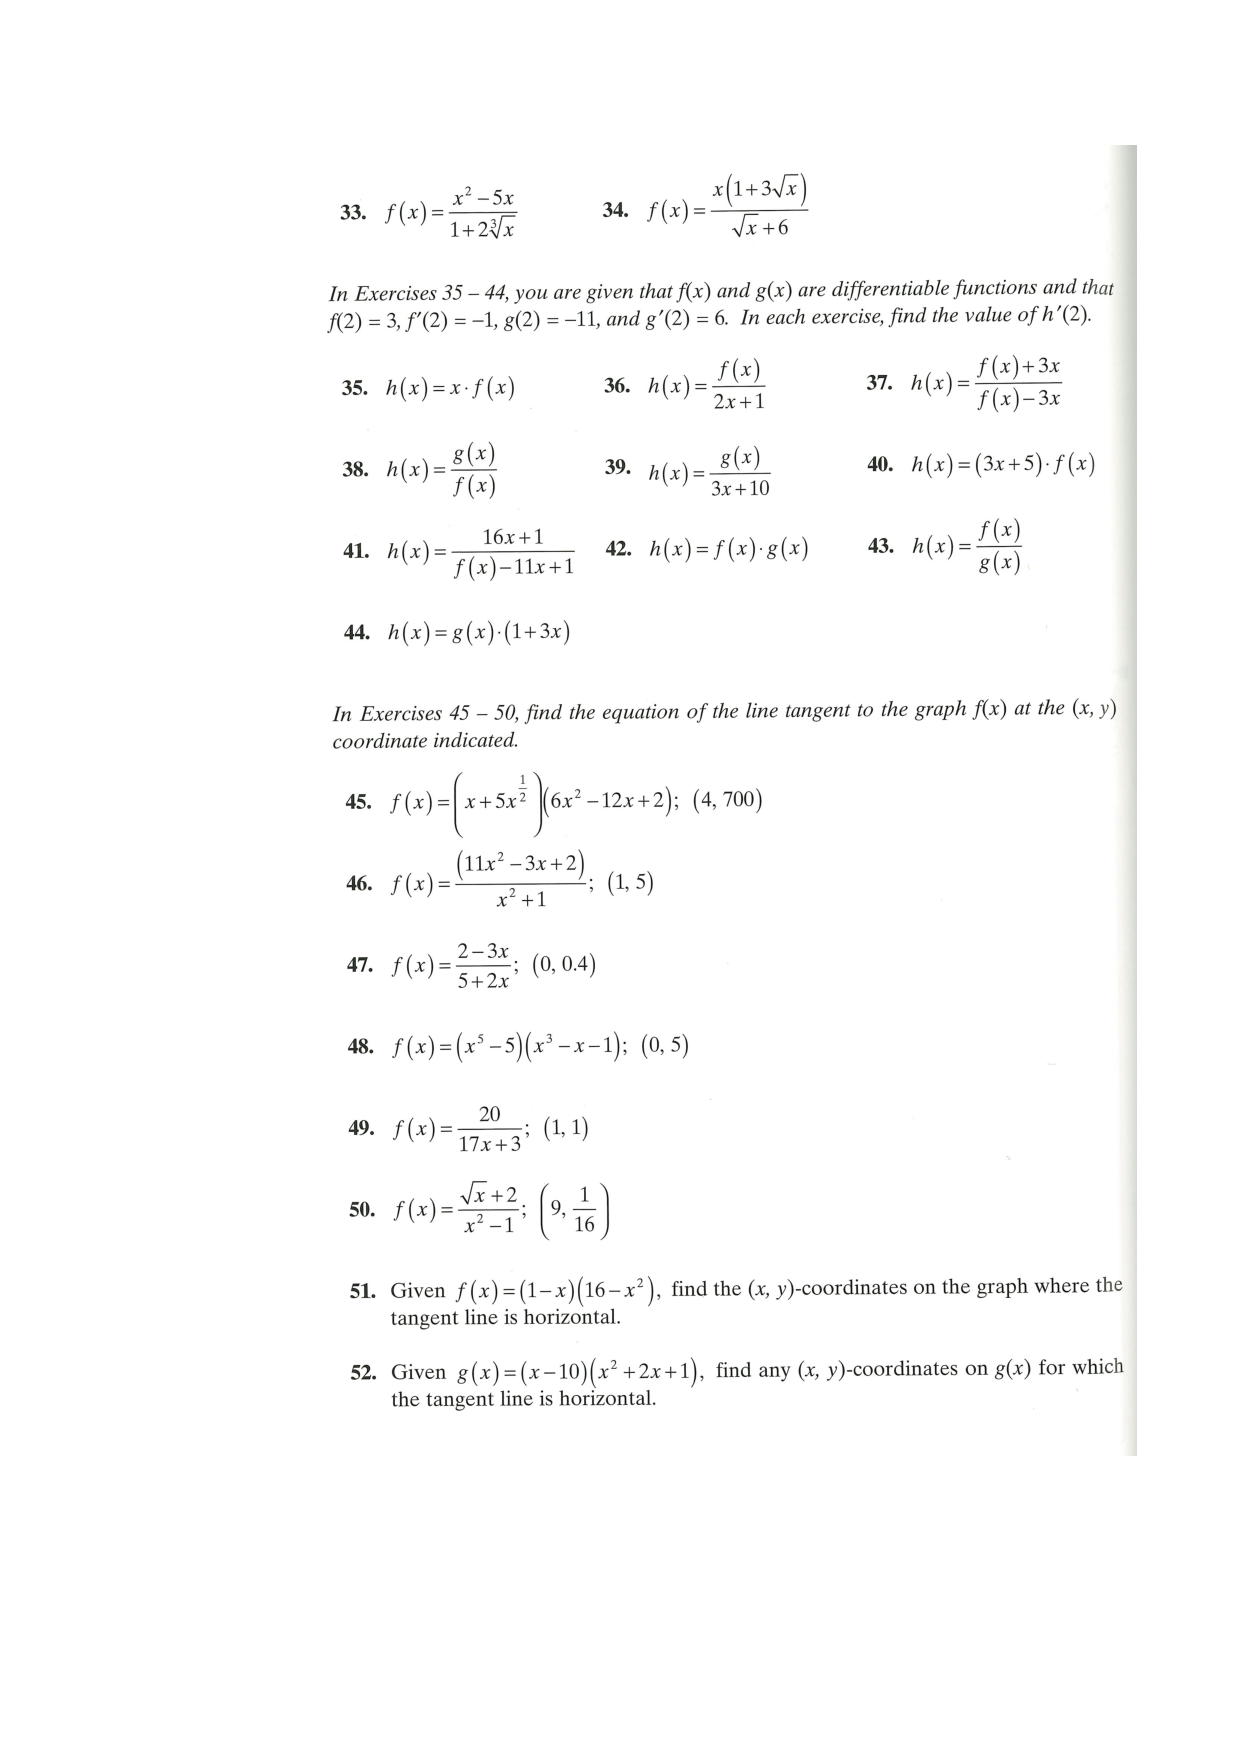
\includegraphics[width=\paperwidth]{\chapdir/0305xB.pdf}}
\newpage
\noindent\makebox[\textwidth]{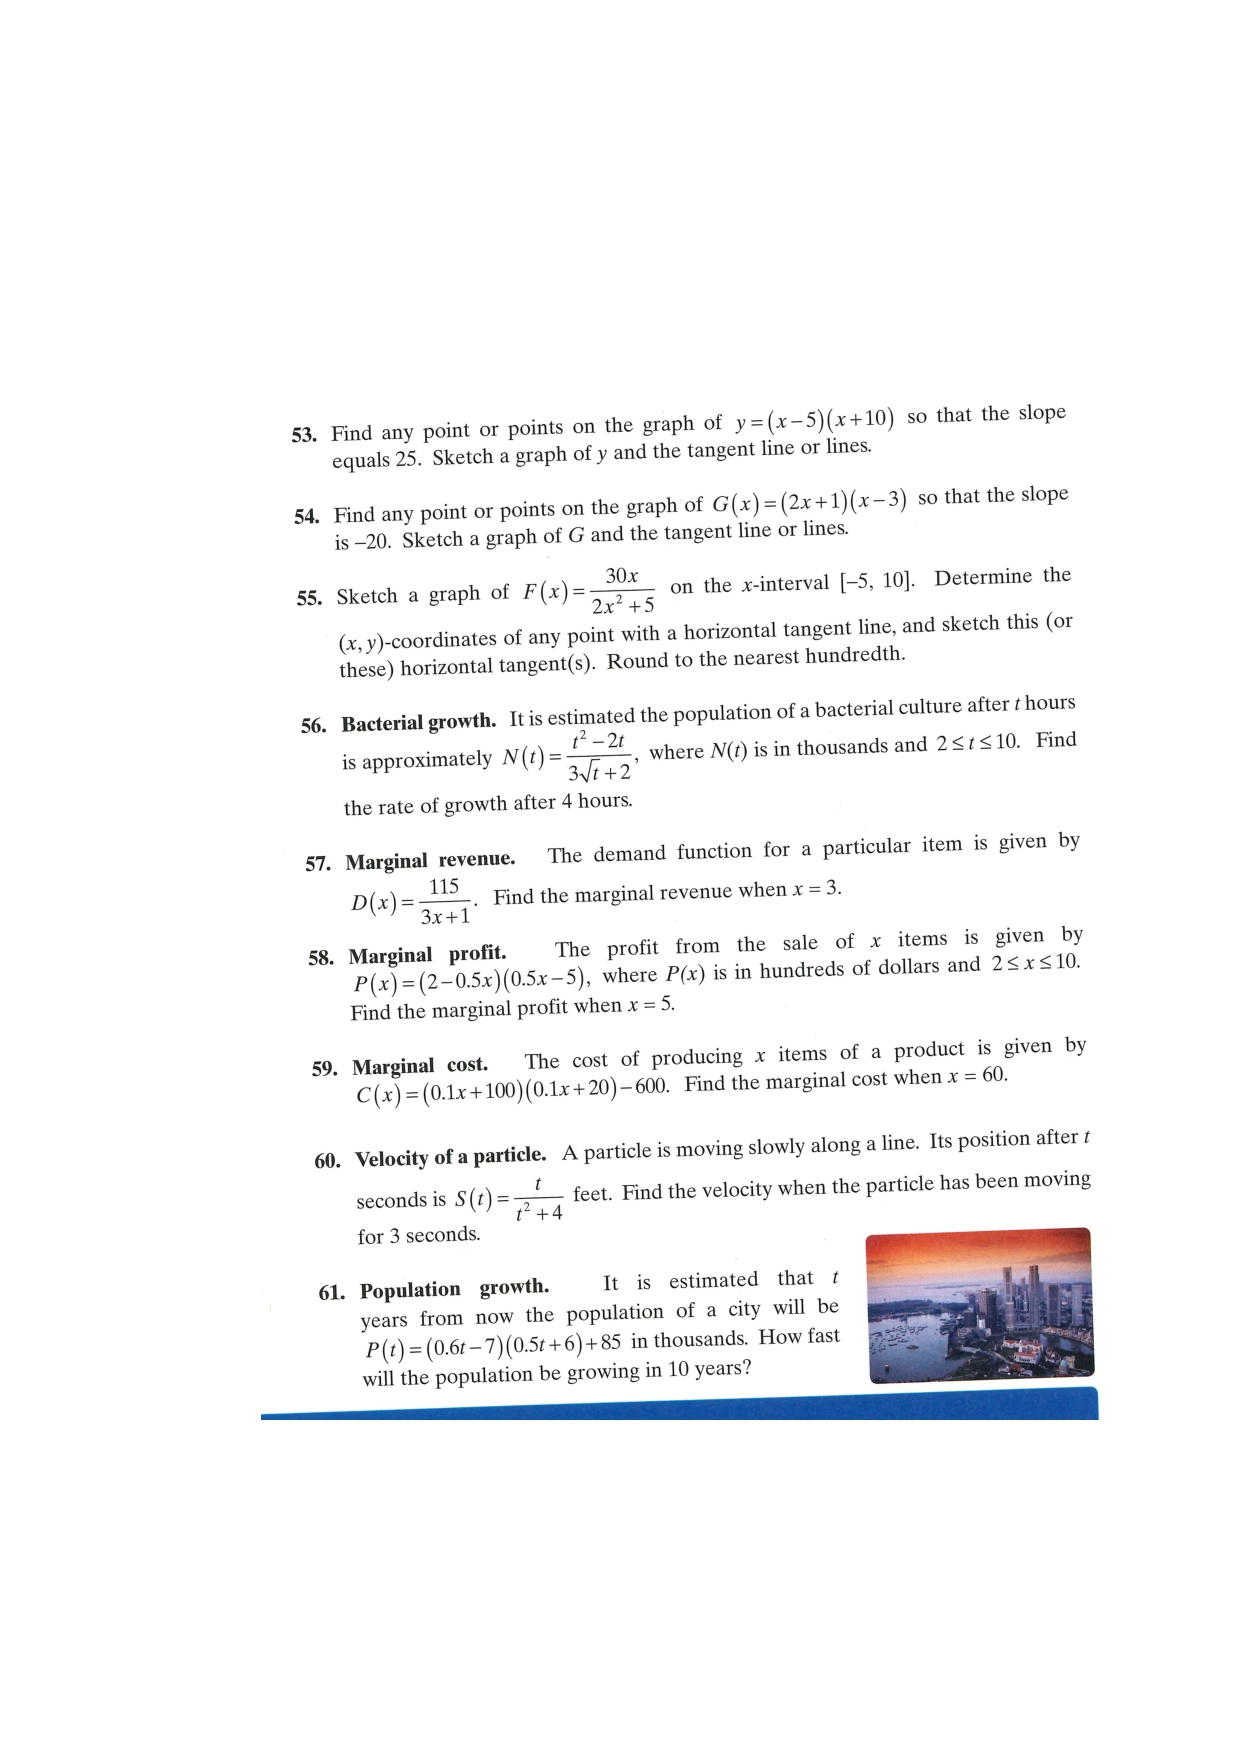
\includegraphics[width=\paperwidth]{\chapdir/0305xC.pdf}}





\newpage

\section{Review}
\subsection{Chapter Review}
We have covered a lot of ground.  The fundamental linearity of many functions serves
as justification for us using the difference quotient on them.  This created new functions which 
described the lines tangent to them at any point.  We have only seen this on function which are
powers of $x$, which can be written as $x^n$, and we saw that the rule of thumb for the
derivative of such equations is $n\cdot x^{n-1}$.
\subsection{Chapter Test}


